\documentclass[11pt, a4paper]{article}
\usepackage[T1]{fontenc}
\usepackage{geometry, microtype}
\usepackage{amsmath, amssymb, mathtools}
\usepackage{bm, physics, siunitx}
\usepackage[shortlabels]{enumitem}
\usepackage{graphicx, wrapfig}
\usepackage{xcolor}
\usepackage{hyperref}

% BEGIN BIBLIOGRAPHY CONFIGURATION
% --------------------------------------------- %
\usepackage[maxcitenames = 2, backend=biber]{biblatex}
\usepackage{../bib/atlasbiblatex}
\addbibresource{../bib/sources.bib}
\renewcommand*{\bibfont}{\small}
% --------------------------------------------- %
% END BIBLIOGRAPHY CONFIGURATION


% BEGIN PACKAGE CONFIGURATION
% --------------------------------------------- %
\graphicspath{{../media}}
\hypersetup{colorlinks = true, allcolors=blue}
\sisetup{separate-uncertainty=true, exponent-product=\cdot}

\newcommand{\hmargin}{3.5cm}
\newcommand{\vmargin}{3.25cm}
\geometry{top=\vmargin, bottom=\vmargin, left=\hmargin, right=\hmargin}
% --------------------------------------------- %
% END PACKAGE CONFIGURATION


% BEGIN HEADER CONFIGURATION
%--------------------------------------------%
\usepackage{fancyhdr, extramarks}
\pagestyle{fancy}

\fancyhf{}
\fancyhead[L]{\textit{\firstrightmark}}
\fancyfoot[C]{\centering \thepage}

\renewcommand{\sectionmark}[1]{
    \markboth{\thesection. \ #1}
    {\noexpand\firstsubsectiontitle}
    \global\firstsubsectionmarktrue}
\renewcommand{\subsectionmark}[1]{
    \markright{\thesubsection. \, #1}
    \iffirstsubsectionmark
\edef\firstsubsectiontitle{\thesubsection. \, #1}
\fi
\global\firstsubsectionmarkfalse}
\newif\iffirstsubsectionmark
\def\firstsubsectiontitle{}
%--------------------------------------------%
% END HEADER CONFIGURATION


% BEGIN CUSTOM MACROS
% --------------------------------------------- %
\definecolor{myMaroon}{RGB}{96,0,6}
\newcommand{\myhref}[2]{\hyperref[#1]{\textcolor{blue}{#2}}}
\newcommand{\myurl}[1]{\textcolor{blue}{\texttt{\url{#1}}}}
\DeclarePairedDelimiter\floor{\lfloor}{\rfloor}  % floor function

\newcommand{\diff}{\mathop{}\!\mathrm{d}}
\renewcommand{\vec}[1]{\bm{#1}}
\newcommand{\mat}[1]{\mathbf{#1}}
\newcommand{\tensor}[1]{\mathsf{#1}}
\newcommand{\uvec}[1]{\hat{\vec{#1}}}
\renewcommand{\grad}{\nabla}

\newcommand{\X}{\mat{X}}
\newcommand{\W}{\mat{W}}
\newcommand{\x}{\vec{x}}
\newcommand{\y}{\vec{y}}
\newcommand{\w}{\vec{w}}
\renewcommand{\b}{\vec{b}}
\newcommand{\z}{\vec{z}}
\renewcommand{\a}{\vec{a}}

\newcommand{\subgrad}[1]{\grad_{\mspace{-4mu}#1}\mspace{1mu}} % gradient with a subscript
\newcommand{\supgrad}[2]{\grad_{\mspace{-4mu}#1}\mspace{1mu}^{\mspace{-4mu}#2}} % gradient with a subscript and superscript
\newcommand{\chem}[1]{\ensuremath{\mathrm{#1}}}  % for typesetting chemical formulas e.g. PbWO_4
% --------------------------------------------- %
% END CUSTOM MACROS


\begin{document}

% BEGIN TITLE PAGE
% --------------------------------------------- %
\thispagestyle{empty}
\begin{center}

    \definecolor{ul-red}{RGB}{220,29,39}
    \begin{figure}[htb!]
        \centering
        
\includegraphics[width=0.1\linewidth]{raster/ul-logo}
    \end{figure}
    \huge{\textsc{University of Ljubljana}}\\
    \LARGE{\textsc{Faculty of {\color{ul-red} Mathematics and Physics}}}\\[1mm]
    \Large{\textsc{Department of Physics}}\\
    \vspace{5mm}
    \huge{Seminar}\\
    \vspace{5mm}
    \rule{\textwidth}{0.2pt}\\[3mm]
    \LARGE{\textbf{End-to-End Classification for Discovery of\\New Processes in High-Energy Physics}}
    % End-to-End Particle Classification for Discovery of New Processes in High-Energy Physics
    \rule{\textwidth}{0.2pt}

    \vspace{5mm}

    % \large{\textit{Prepared by}: Elijan Jakob Mastnak}\\
    % \large{\textit{Adviser}: prof. dr. Borut Paul Ker\v{s}evan}

    \begin{minipage}[t]{0.90\textwidth}
        \normalsize{\textsc{Author:}} \hfill \large{\textsc{Adviser}:}\\
    \large{Elijan Jakob Mastnak} \hfill \large{prof. dr. Borut Paul Ker\v{s}evan}
    \end{minipage}

\end{center}

\vspace{10mm}
% add myurl links to all sources
\begin{center}
    \textbf{Abstract}\\[2mm]
    \begin{minipage}[t]{0.85\textwidth}
        This work explores the use of convolutional neural networks to classify the products of high-energy particle collisions using low-level, image-based detector data. We restrict ourselves to binary classification, and, for concreteness, focus on the popular example of distinguishing Higgs boson and background events. We begin by defining end-to-end classification, explain how the data used to perform this classification is measured at the Large Hadron Collider, and outline how both fully-connected and convolutional neural networks use this data to perform classification. We conclude by presenting a concrete study involving image-based end-to-end classification, and compare end-to-end workflows to traditional classification methods based on reconstructed kinematic features.
    \end{minipage}

    \vspace{10mm}
    \large{Ljubljana, May 2021}
\end{center}
% --------------------------------------------- %
% END TITLE PAGE

\newpage
\thispagestyle{empty}
\tableofcontents 
\newpage

\section{Why End-to-End Classification?}
\subsection{What is Particle Classification?}
Before discussing the merits of one classification method or the other, we must first define what we mean by classification. For our purposes, particle classification answers the following question:
\begin{quote}
    ``Two high-energy particles collide. Which particles were produced as a result of their collision?''
\end{quote}
    For concreteness, we will focus on binary classification involving Higgs boson detection, in which we consider only two possible outcomes. These are:
\begin{enumerate}

    \item a particle collision produced a Higgs boson (\textit{signal}), or

    \item a collision produced anything other than a Higgs boson (\textit{background}).

\end{enumerate}

\subsection{Why End-to-End Classification?}

\begin{figure}[htb!]
        \centering
        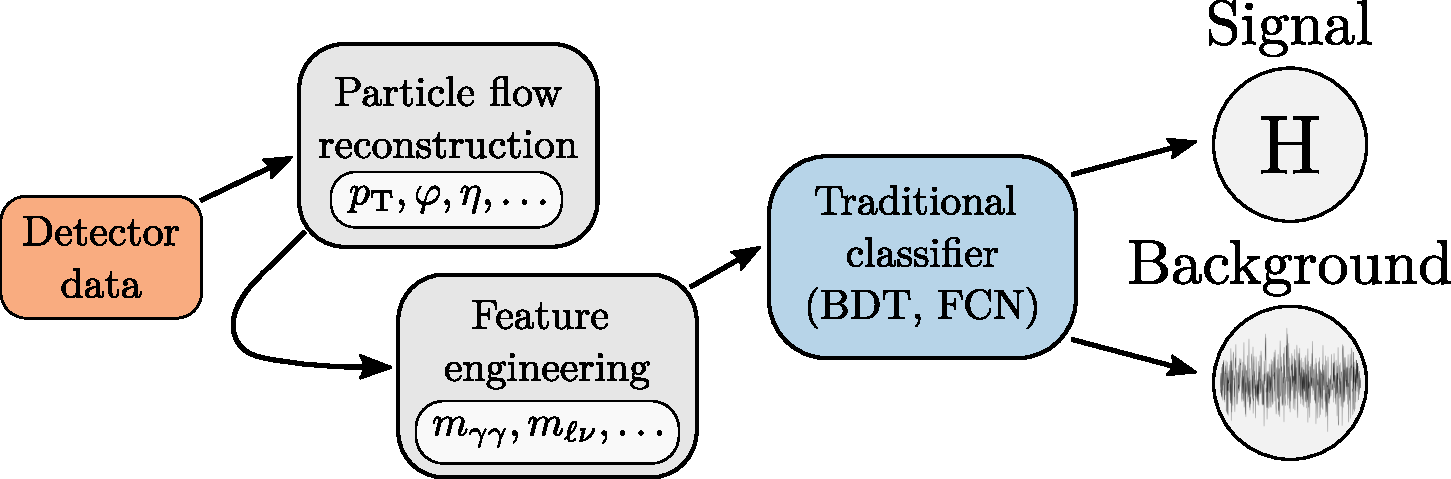
\includegraphics[width=0.8\linewidth]{vector/traditional-pipeline.pdf}
        \caption{An abstracted traditional particle classification workflow.}
        \label{fig:traditional-pipeline}
\end{figure}

Perhaps the best motivation for ``end-to-end'' classification comes from showing, as in Figure \ref{fig:traditional-pipeline}, what end-to-end classification is \textit{not}. In particular, the steps ``Particle flow reconstruction'' and ``Feature engineering'', outlined in \myhref{ss:three-methods}{Section \ref{ss:three-methods}}, turn out to be quite non-trivial. End-to-end classification removes these steps. In an end-to-end workflow, shown schematically in Figure \ref{fig:cnn-pipeline}, a classifier outputs a result computed directly from raw detector data, with minimal intermediate data processing.

\begin{figure}[htb!]
    \centering
    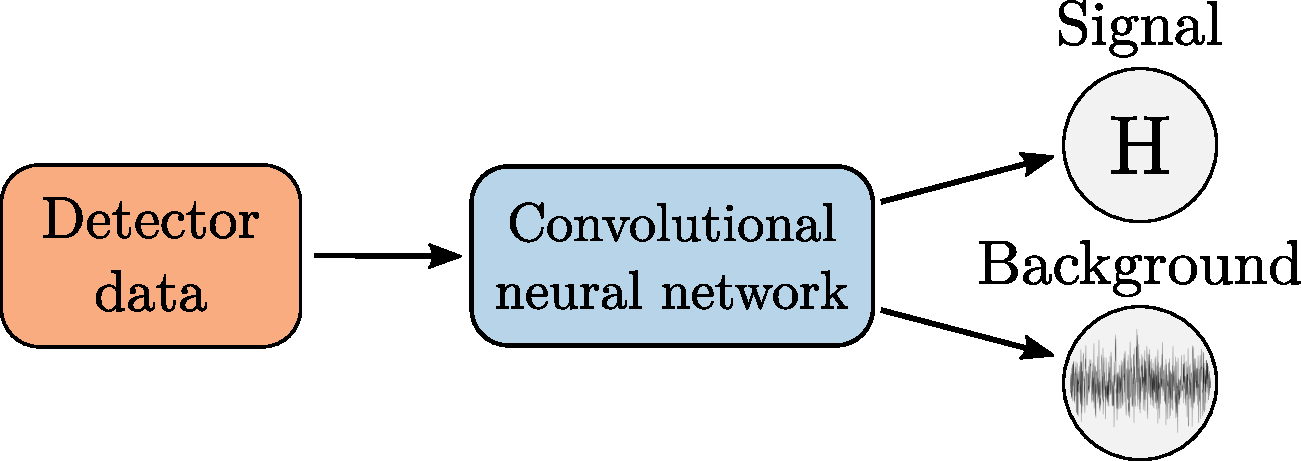
\includegraphics[width=0.70\linewidth]{vector/cnn-pipeline.pdf}
    \caption{An end-to-end classification workflow eliminates the complicated intermediate steps involved in traditional classification (cf. Figure \ref{fig:traditional-pipeline}).}
    \label{fig:cnn-pipeline}
\end{figure}

 As implied by Figures \ref{fig:traditional-pipeline} and \ref{fig:cnn-pipeline}, particle classification requires data measured by a particle detector. In the next section, we explore the nature of this detector data, and outline how the data is produced and measured at the Large Hadron Collider.

\section{How the LHC Produces and Measures Collision Data}
For our purposes, the Large Hadron Collider (LHC) is a synchrotron accelerator that collides protons at teravolt-order center-of-mass energy \cite{lhc}. Each collision produces a cascade of secondary particles, whose energies and trajectories are measured in specialized detectors like CMS and ATLAS. The purpose of this section is to explain:
\begin{enumerate}

    \item the process leading up to a proton collision at the LHC,

    \item the physical principles behind a detector's measurement instruments, and
    % how the detector measures the energy and trajectories of the collision's decay products, and

    \item the image-like format of low-level detector data used by end-to-end classifiers. % used by neural networks for particle classification.

    % \item how the pixels and colors in Figure \ref{fig:data-raw-ecal} correspond directly to the energies and trajectories of physical particles in an actual collision event.

\end{enumerate}

\subsection{The CERN Accelerator Chain}

\begin{figure}[htb!]
    \centering
    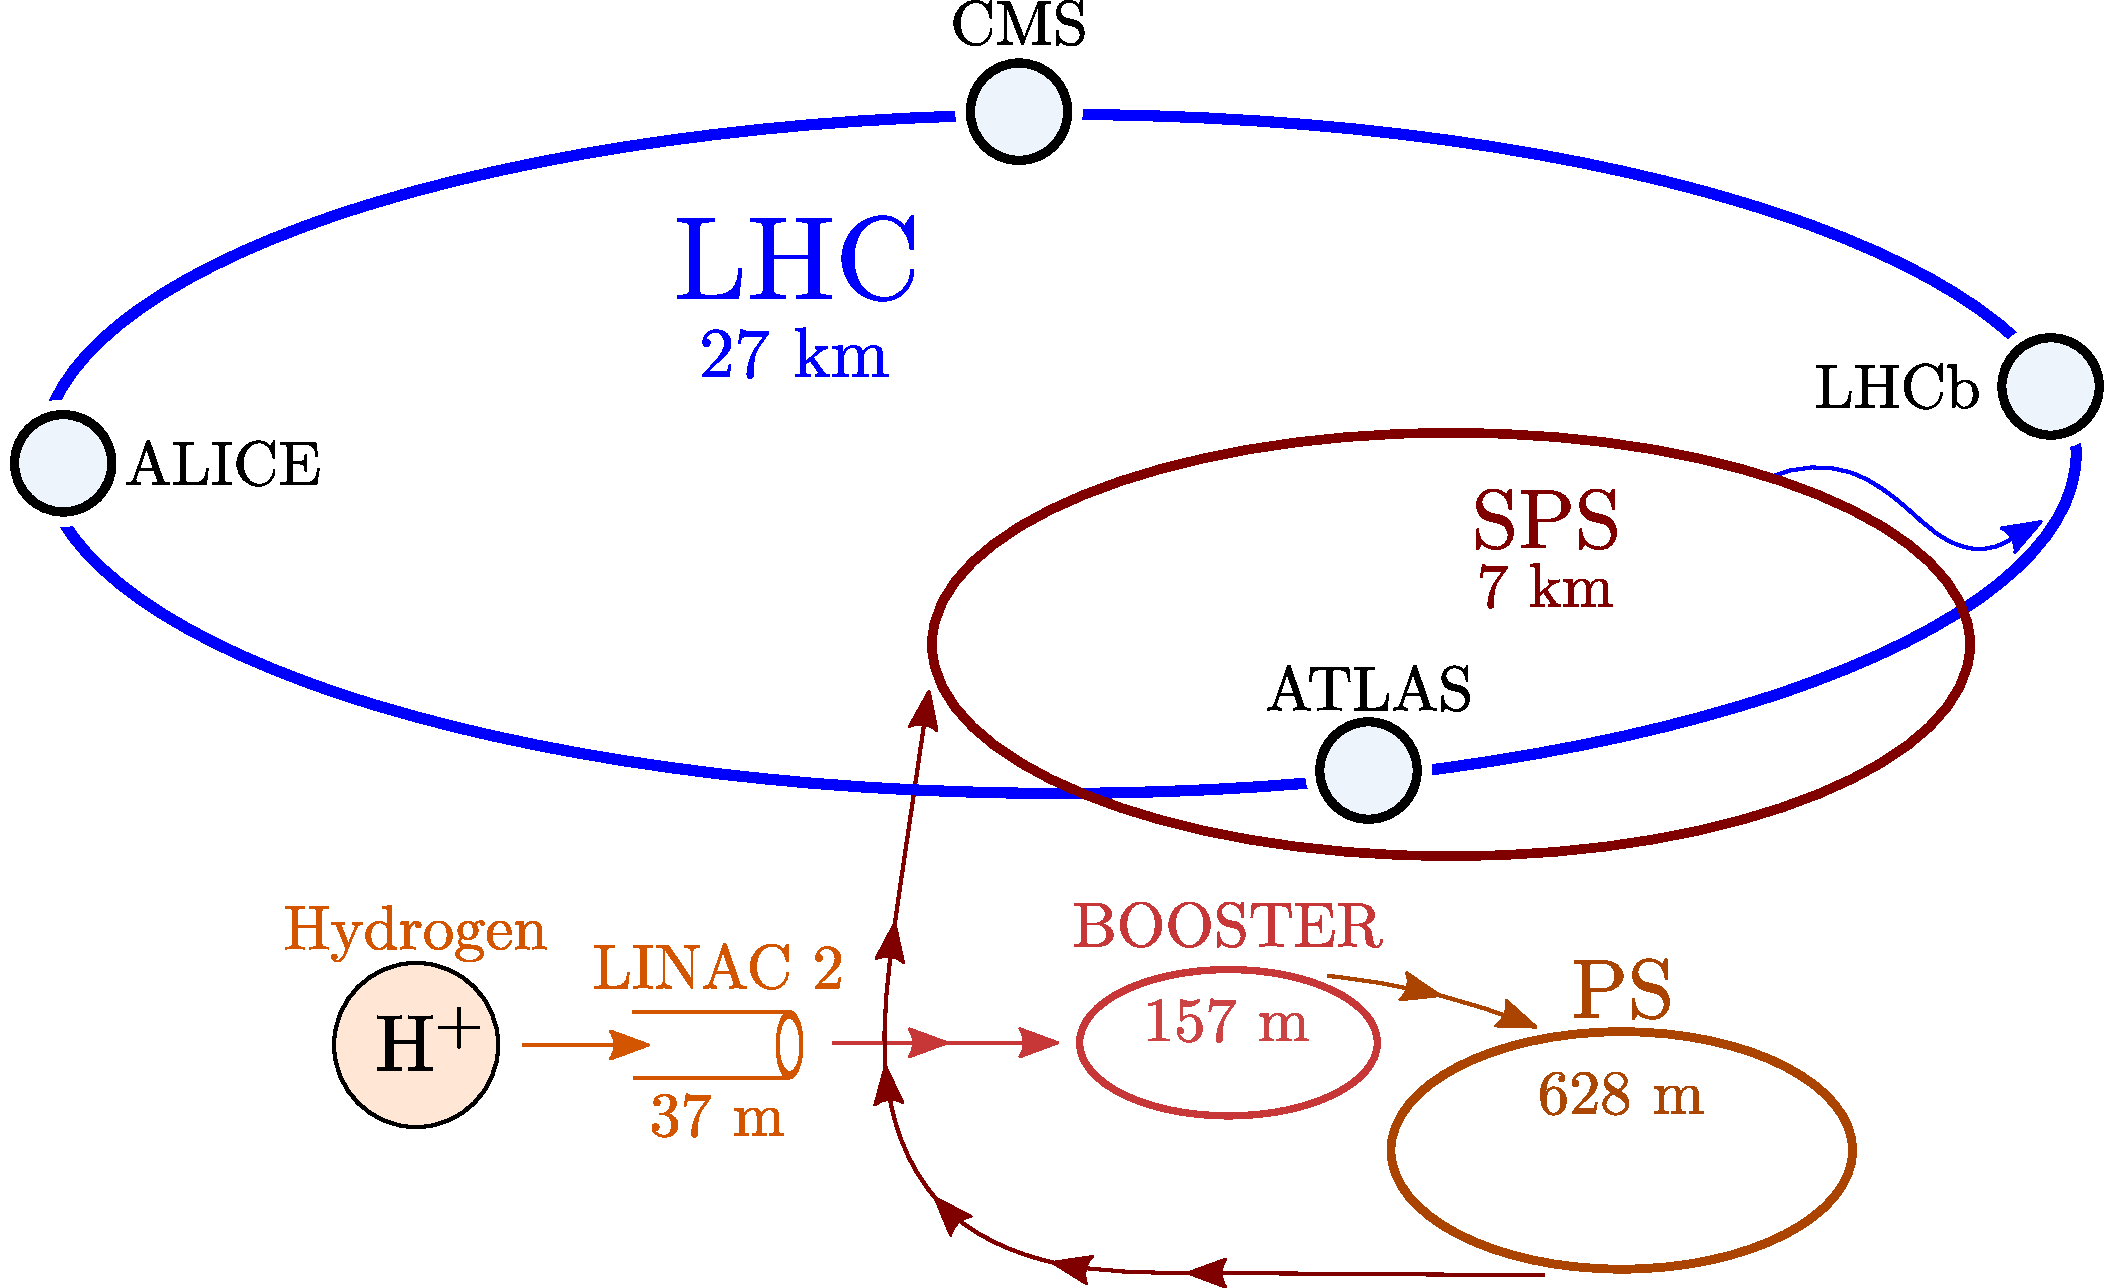
\includegraphics[width=0.75\linewidth]{vector/cern-complex.pdf}
    \caption{The components of the CERN accelerator complex relevant to this work. Adapted from \cite{image-cern-complex}.}
    \label{fig:cern-complex}
\end{figure}

The story begins with a bottle of hydrogen gas. A strong electric field strips the hydrogen atoms of their electrons, leaving behind only protons. These protons are accelerated through the linear accelerator \textit{Linac2},\footnote{In the LHC's 2020 high luminosity upgrade, Linac2 is replaced with Linac4, which accelerates negative hydrogen ions instead \cite{linac4-tdr}.} setting in motion a journey through the maze of synchrotron boosting stages shown in Figure \ref{fig:cern-complex} and culminating at the LHC. Depending on operating conditions, the LHC accelerates protons to an ultimate kinetic energy of up to \SI{6.5}{\tera \electronvolt}; these protons travel around the LHC in two opposing beamlines in bunches of roughly $ 10^{11} $ particles, separated in time by \SI{25}{\nano \second}. The beamlines cross, allowing for proton-proton collisions, at four nominal collision points, around which are centered, in anticipation, the LHC's four main detectors: ALICE, CMS, LHCb, and ATLAS.

\subsection{Collision and Detection}
Most protons in opposing beams zoom past each other without appreciable interaction. Rarely, however, two protons collide head-on, setting in motion a chain of interactions which ultimately produces a cascade of familiar elementary particles such as electrons, protons, neutrons, muons, photons, and neutrinos. These secondary particles are collectively called the collision's \textit{decay signature}, and fly outward in all directions from the primary collision point through a surrounding particle detector. This brings us to a key concept:
\begin{quote}
    The exotic particles of interest in high-energy physics (e.g. a Higgs boson) decay far, far before they can interact with the detector. The detector measures only the secondary particles further down the decay chain.
\end{quote}
In other words, \textit{we have no way of detecting a Higgs boson directly. The best we can do is infer its presence from the nature of the collision's decay signature}. Thus, to progress, we need a quantitative description of a decay signature.


\subsection{Quantifying a Decay Signature} \label{ss:quantify-decay}
Fundamentally, a particle detector measures the following decay signature properties:
\begin{enumerate}

    \item the trajectory of particles through the detector, and

    \item the energy deposited in the detector by detected particles.

\end{enumerate}
Trajectories are measured with instruments called \textit{trackers}, while energy is measured with \textit{calorimeters}. From trajectory and energy, and by noting which particles appear in which subdetector, we can reconstruct a number of secondary quantities, including particle momentum, identity, and the positions of production and decay vertices. In this section we first define the detector coordinate system, then discuss each measurement instrument in turn. For concreteness, we will focus on the instruments used at the Compact Muon Solenoid (CMS) detector \cite{cms}, but similar concepts apply to most particle detectors currently used in high-energy physics. For better orientation, each of the four CMS sub-detectors discussed in this section appear, in correct scale, in the diagram of the CMS detector shown in Figure \ref{fig:cms} two pages below.

\subsubsection{The Detector Coordinate System at the CMS}
The CMS coordinate system is best understood visually, as shown in Figure \ref{fig:cms-coordinate-system}. The detector uses a hybrid Cartesian/cylindrical coordinate system, in which the origin coincides with the nominal collision point, while the $ x $, $ y $, and $ z $ axes point towards the center of the LHC, vertically upward, and along the beamline, respectively. The azimuthal angle $ \varphi $ is measured in the $ xy $ plane, while the polar angle $ \theta $ is measured in the $ yz $ plane. Conventionally, the polar angle is given in terms of a quantity called \textit{pseudorapidity},\footnote{Particle physicists work with pseudorapidity, and a related quantity called rapidity, because differences in these quantities are Lorentz-invariant to boosts along the beam axis. For our purposes, it is enough to view pseudorapidity as just an alternate representation of the polar angle $ \theta $.} denoted by $ \eta $ and defined as
\begin{equation}
    \eta \equiv - \ln \left( \tan \frac{\theta}{2} \right) \implies \theta = 2 \arctan e^{- \eta}. \label{eq:pseudorapidity}
\end{equation}

\begin{figure}[htb!]
    \centering
    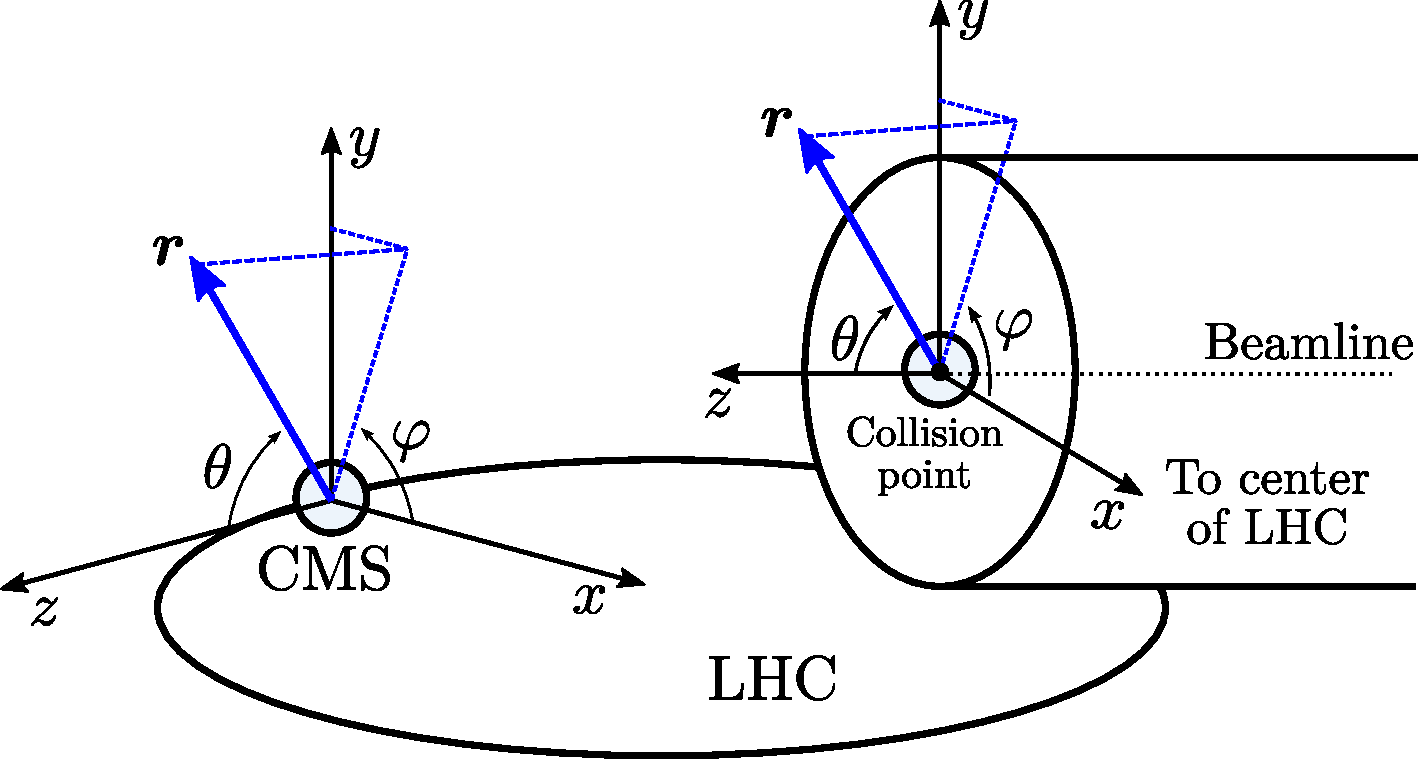
\includegraphics[width=0.9\linewidth]{vector/cms-coordinate-system.pdf}
    \caption{Two perspectives of the coordinate system used at the CMS detector.}
    \label{fig:cms-coordinate-system}
\end{figure}

\subsubsection{Trackers}
Trackers measure the trajectory (position with respect to time) of particles flying out from the collision point. The basic tracker building blocks are microscopic silicon pixels and strips with dimensions of order \SIrange{10}{100}{\micro \meter}, each connected to its own electronic read-out channel. Each pixel (strip) has an intrinsic electric field, similar in principle to the built-in electric field in a pn junction's depletion region.

The CMS tracker \cite{tracker-tdr} consists of millions of these silicon elements arranged in concentric, cylindrical layers around the nominal collision point. An incident particle passing through a silicon pixel (strip) excites the atoms in the pixel's (strip's) depletion region, creating electron-hole pairs. The silicon element's electric field then accelerates the electrons and holes to opposite pixel (strip) faces, leading to a measurable charge pulse called a \textit{hit}. Hits from successive layers are combined to reconstruct an incident particle's trajectory. 

Importantly, the CMS tracker is immersed in a \SI{4}{\tesla} magnetic field, generated by the CMS's namesake \textit{solenoidal} superconducting magnet. Because of this magnetic field, charged particles in the Tracker bend under the influence of the Lorentz force, which allows physicists to reconstruct the momenta of charged particles from the curvatures of their Tracker trajectories.


\subsubsection{Electromagnetic Calorimeters}
Electromagnetic calorimeters (ECALs) measure the energy of particles that interact with matter via the electromagnetic interaction. At the CMS, the basic ECAL building block is a lead tungstate (\chem{PbWO_4}) scintillator crystal connected to a photodetector \cite{ecal-tdr}.

The basic working principle is as follows: high-energy incident particles interact with the \chem{PbWO_4} scintillators (electrons via bremsstrahlung, high-energy photons predominantly via pair production) to produce secondary \textit{electromagnetic showers}---cascades of lower-energy photons, electrons, and positrons. Shower particles excite the \chem{PbWO_4} scintillators, which emit blue-light \textit{scintillation photons} during the relaxation process. These scintillation photons reach the crystal's attached photodetector (avalanche photodiodes in the ECAL barrel and vacuum phototriodes in the ECAL end caps \cite{ecal-tdr}), where they free electrons via the photoelectric effect. After further amplification, these photoelectrons produce a measurable electric current whose amplitude encodes the energy deposited by the initial incident particle.

\begin{figure}[htb!]
    \centering
    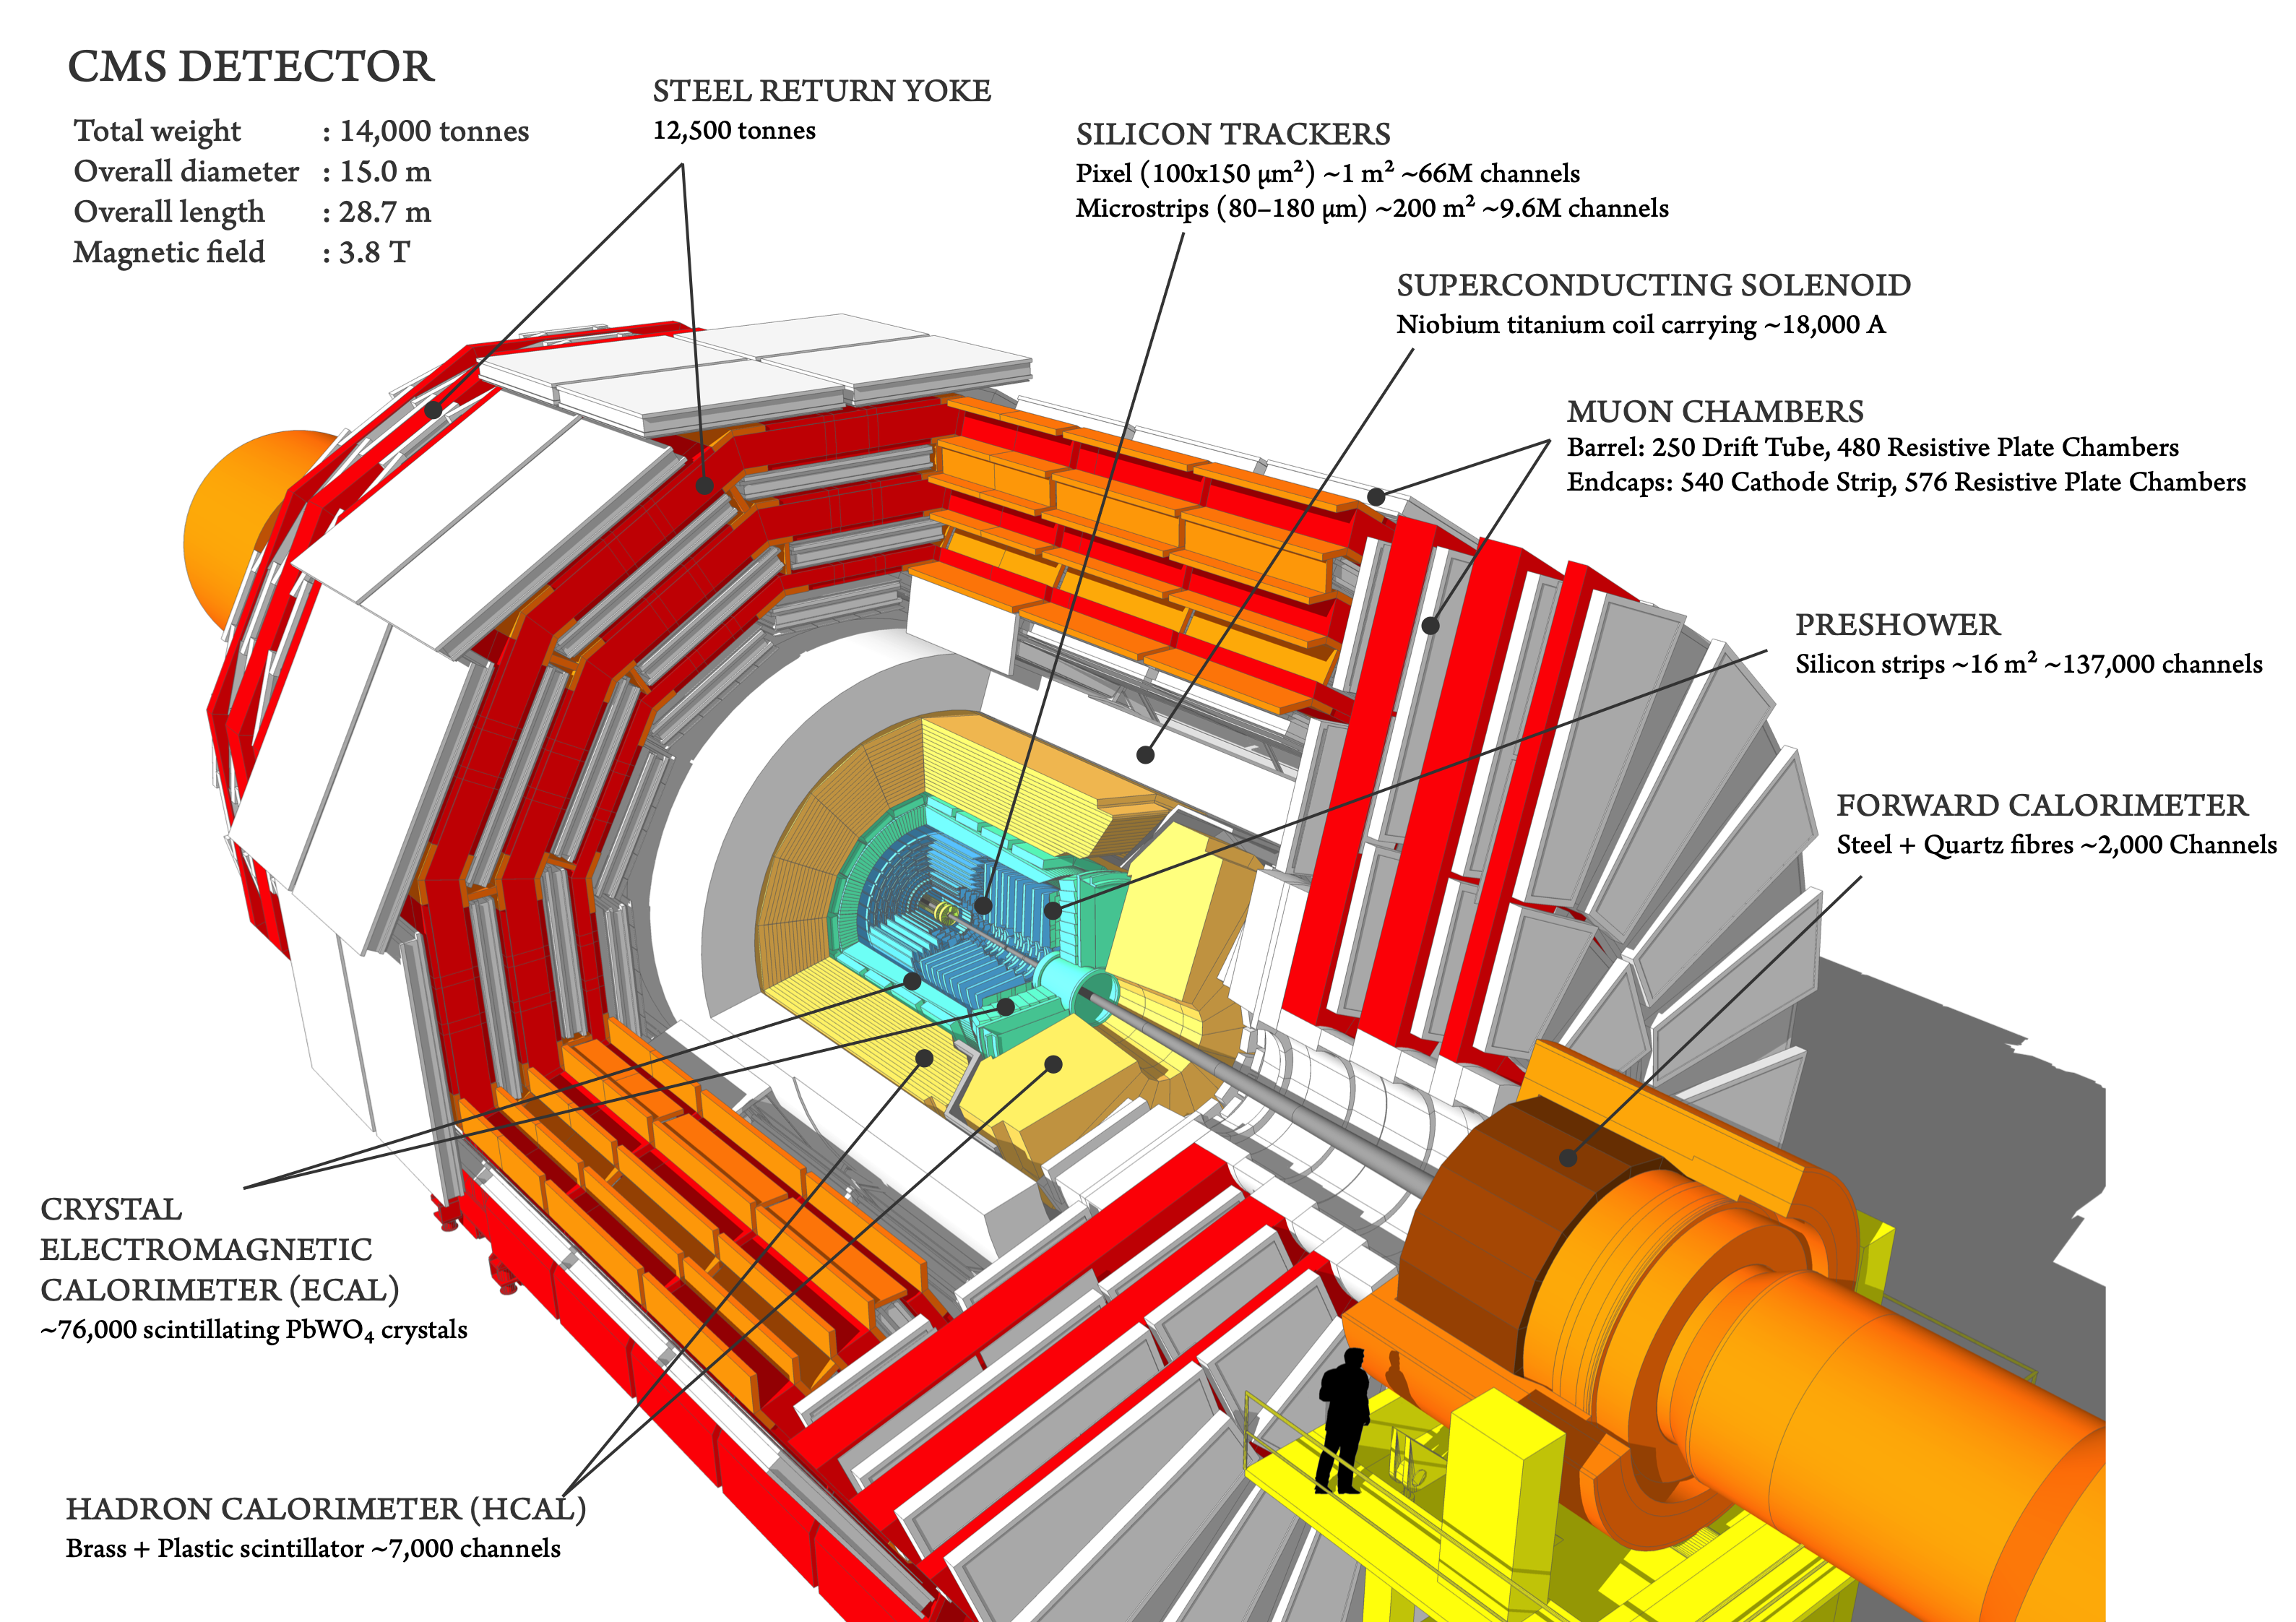
\includegraphics[width=0.9\linewidth]{raster/png/cms.png}
    \caption{A cutaway diagram of the CMS detector, showing each of the sub-detectors (silicon trackers, ECAL, HCAL, and muon detectors) discussed in this work. \cite{image-cms}}
    \label{fig:cms}
\end{figure}

\subsubsection{Hadronic Calorimeters}
Hadronic calorimeters (HCALs) measure the energy of particles that interact with matter via the strong interaction. The CMS HCAL consists of alternating layers of absorbers---brass and steel plates---and scintillation detection modules---plastic scintillator tiles connected to hybrid photodiodes \cite{hcal-tdr}.

A high-energy particle interacts with the absorber material, primarily via the strong interaction, to produce a \textit{hadronic shower}---a cascade of lower-energy hadronic particles. The shower particles excite the plastic scintillator tiles, which emit blue-light scintillation photons; these photons are then converted to a measurable electric current via the photoelectric effect by the tiles' attached photodiodes. Just like in the ECAL, the current's amplitude encodes the energy deposited by an incident particle, while the position of the activated scintillator tile encodes the particle's position.

\subsubsection{Muon Detection}
For the purposes of this work, this section may be skipped without loss of continuity. However, for completeness, we now briefly outline the CMS's namesake muon detection system. The CMS muon detector is a gas-based detector, whose basic module is a rectangular \textit{drift tube} enclosing a mixture of argon and \chem{CO_2} gas (10 to 20 percent \chem{CO_2} by volume). Through the chamber's center runs a thin steel anode wire (radius \SI{50}{\micro \meter}), held at a kilovolt-order potential difference relative to copper-coated electrodes glued to the chamber's outer surface \cite{muon-tdr}.

A high-energy muon incident on the drift tube ionizes the internal gas, freeing electrons and positive ions. These ions are accelerated across the tube's potential difference to the anode wire and cathode electrodes, respectively, resulting in a measurable pulse of electric charge. The number of freed ions is proportional to the energy deposited in the drift tube by the incident muon, so the signal amplitude, like in ECAL and HCAL, encodes the muon's energy; the location of the signal pulse along the electrodes reveals the muon's position. 

Three other muon detector components, namely resistive plate chambers, cathode strip chambers, and gas electron multipliers, rely on the same physical principle of gas ionization and ion collection. For more information, interested readers are referred to Refs. \cite{muon-web} or \cite{muon-tdr} for a friendly or technical discussion, respectively.

Importantly, the muon detection system resides at the very outer layer of the CMS. Since muons are the only familiar decay product (besides neutrinos, which do not ionize gas) to pass through the ECAL and HCAL unimpeded, we can be reasonably sure any particle registered in the muon detector is indeed a muon.

\subsection{Low-Level Detector Data and How It Is Used} \label{ss:three-methods}

\begin{figure}[htb!]
    \centering
    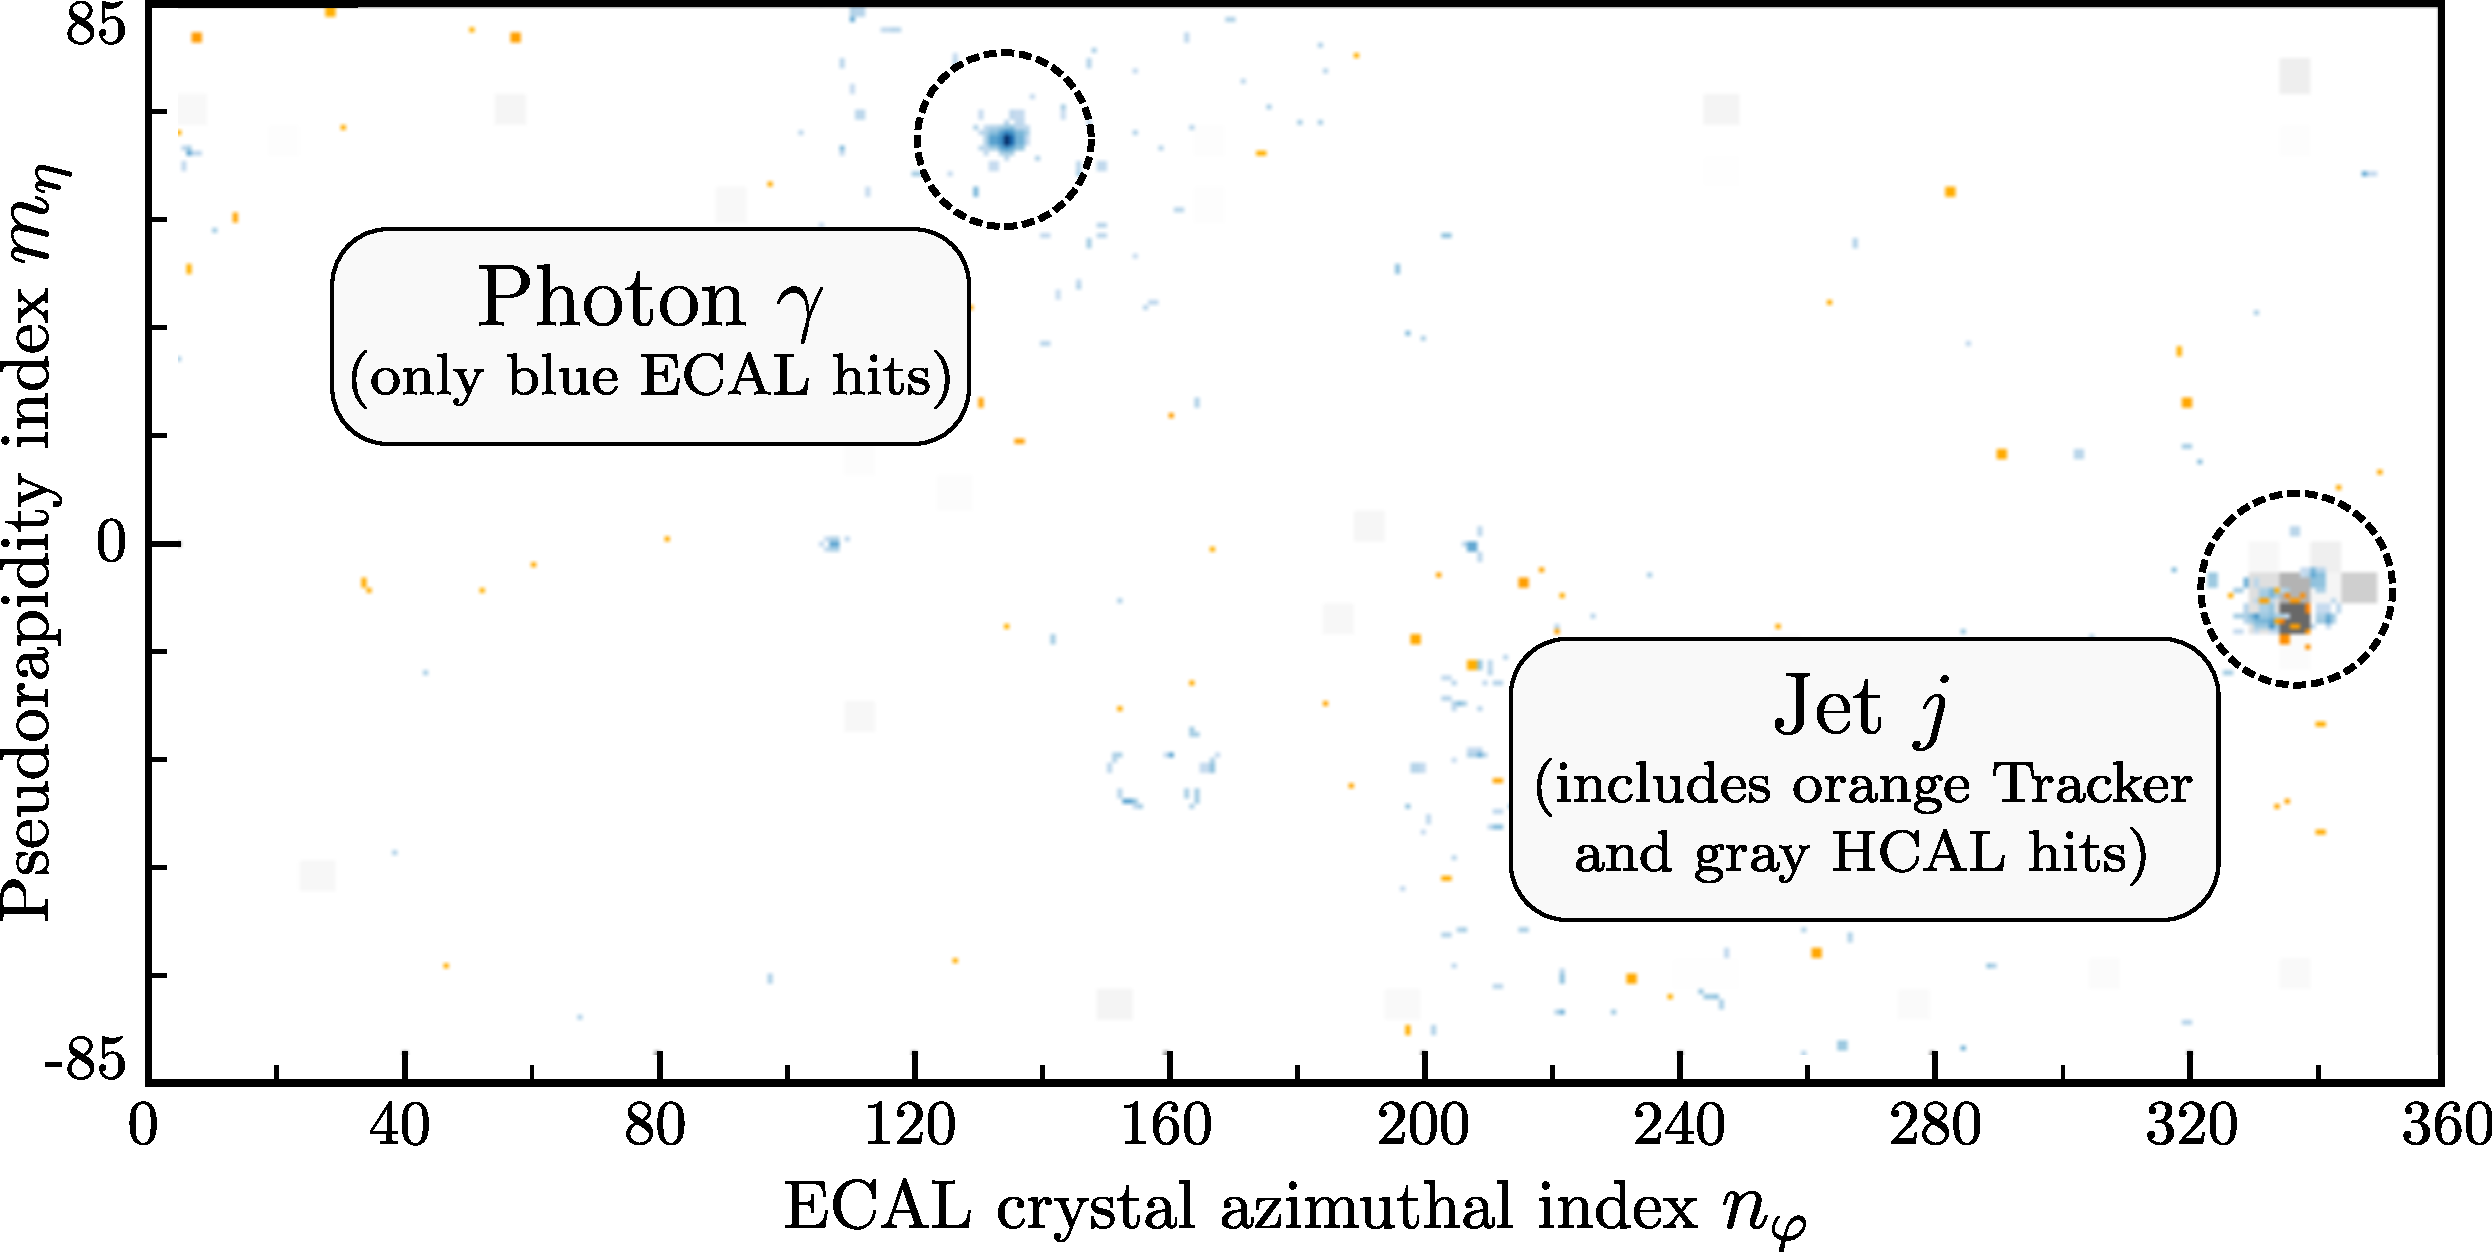
\includegraphics[width=\linewidth]{raster/raster-svg/event-image.pdf}
    \caption{A composite image of a photon+jet (background) event at the CMS. Tracks appear in orange log scale, ECAL hits in blue log scale, and HCAL hits in gray linear scale. Pixels correspond to physical \chem{PbWO_4} scintillator crystals in the ECAL barrel's $ 360 \times 170 $ crystal grid, which spans $ \varphi \in [0, 2\pi) $ and $ \abs{\eta} < 1.479$. Adapted from \cite{andrews-higgs}.}
    \label{fig:data-raw-ecal}
\end{figure}

If we combine the Tracker hits and ECAL/HCAL signal pulses and project these quantities onto the detector's $ \varphi \eta $ plane, we get something like the image shown in Figure \ref{fig:data-raw-ecal}. This image, from a simulated photon+jet event at the CMS \cite{data-bg-jet}, shows the raw Tracker (position) and ECAL/HCAL (energy) information encoding the event, projected onto the ECAL barrel's $ 360 \times 170 $ grid of \chem{PbWO_4} scintillator crystals. 

Figure \ref{fig:data-raw-ecal} serves as our basic model of low-level detector data: an image-like grid with two spatial dimensions $ (\varphi, \eta) $ and three detector channels, in which pixel intensity corresponds to either (i) charge deposited in the Tracker, or (ii) energy deposited in ECAL or HCAL. In each case, the position of a given pixel in the image has a well-defined physical correspondence to the position of a measurement module (e.g. Tracker pixel, ECAL scintillation crystal) in the detector. Equipped with this form of image-based data, we have three options:
\begin{enumerate}[(a)]

    \item \textit{End-to-end classification}: use the low-level data as is, and feed this data into a convolutional neural network, which outputs a predicted classification result.

    \item \label{item:kinematic-classification} \textit{Kinematic-based classification}, in which we feed the raw data into a \textit{particle flow reconstruction} algorithm,\footnote{Particle flow reconstruction falls largely beyond the scope of this work. As an example, we can reconstruct a particle's transverse momentum from the curvature of its trajectory in the detector's magnetic field, but we will otherwise treat reconstruction as a ``black box'' that outputs kinematic quantities describing a collision. Interested readers are referred to Ref. \cite{particle-flow}.} which reconstructs \textit{kinematic features}, for example transverse momentum (relative to the beam axis) and pseudorapidity (Eq. \ref{eq:pseudorapidity}), describing the decay products. We then use this kinematic data as input into a fully-connected neural network (FCN), which outputs a classification result. 

    \item \label{item:high-level-classification} Reconstruct kinematic features from the low-level data as above, then use these kinematic features to hand-engineer \textit{high-level features}, manually designed to separate signal from background events on an experiment-by-experiment basis (for example, decay particle invariant masses at which we expect high signal production). Then, feed these high-level features, often in combination with the kinematic features described above, into a FCN or BDT classifier. See Ref. \cite{baldi-higgs} for a study comparing kinematic-based and high-level classification.% , which outputs classification results.

    % In practice, high-level features are usually invariant masses of decay particles, for particular values of which we expect a signal peak on theoretical grounds.

\end{enumerate}

Schematically, classification workflows \ref{item:kinematic-classification} and \ref{item:high-level-classification} resemble Figure \ref{fig:fcn-in-out}.
\begin{figure}[htb!]
    \centering
    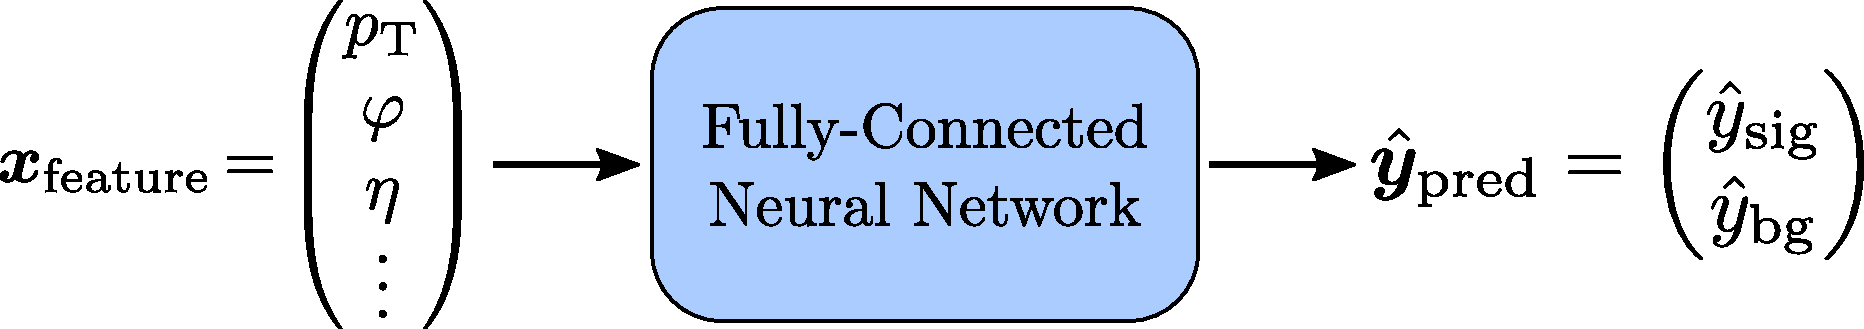
\includegraphics[width=0.9\linewidth]{vector/fcn-in-out.pdf}
    \caption{The binary classification process using a FCN. The outputs $ \hat{y}_{\text{sig}} $ and $ \hat{y}_{\text{bg}} $ represent the predicted probabilities that the inputted feature vector $ \vec{x}_{\text{feature}} $ corresponds to either signal or background, respectively, as explained in \myhref{ss:output}{Section \ref{ss:output}}.}
    \label{fig:fcn-in-out}
\end{figure}

% Understanding the principles of a FCN will provide a firm foundation for understanding the convolutional neural networks used for end-to-end classification.

\section{Fully-Connected Networks} \label{s:fcn}
In this section we take a look inside the ``Fully-Connected Neural Network'' box in Figure \ref{fig:fcn-in-out}. Suppose, as in Figure \ref{fig:fcn-in-out}, that we have a set of kinematic properties encoding a collision event (found, for example, with the particle flow reconstruction algorithm mentioned in \myhref{ss:three-methods}{Section \ref{ss:three-methods}}), which we pack into a vector $ \vec{x} $. In machine learning terminology \cite{homl}, each individual kinematic property is called a \textit{feature}, and the two possible outcomes (signal or background) are called \textit{classes}. The correct class (either signal or background) for a given event is called the event's \textit{target} or \textit{label}, and the complete set of features describing a single event, together with the label, is called an \textit{instance}. Finally, the complete set of available instances (the complete set of collision events) forms a \textit{dataset}. With the vocabulary lesson out of the way, we are equipped to formally describe a neural network. But first, we should reveal supervised machine learning's dirty secret:
\begin{quote}
The dataset used to train a neural network is entirely \textit{simulated}.\footnote{Simulated collision data is constructed with sophisticated algorithms involving Monte-Carlo sampling, a theoretical physical framework such as the Standard Model, and a geometrical model of the particle detector. Like particle flow reconstruction, this falls beyond the scope of this work.}
\end{quote}
Why? Well, we \textit{know} the outcome of each simulated collision event. Thus, our dataset comes with correct labels for every single instance. Using this large dataset of correctly-labeled data, we can train a neural network to give accurate results even when, as in practical applications, the correct results aren't known beforehand. 

\subsection{Understanding a Binary Classifier's Output} \label{ss:output}

\begin{figure}[htb!]
    \centering
    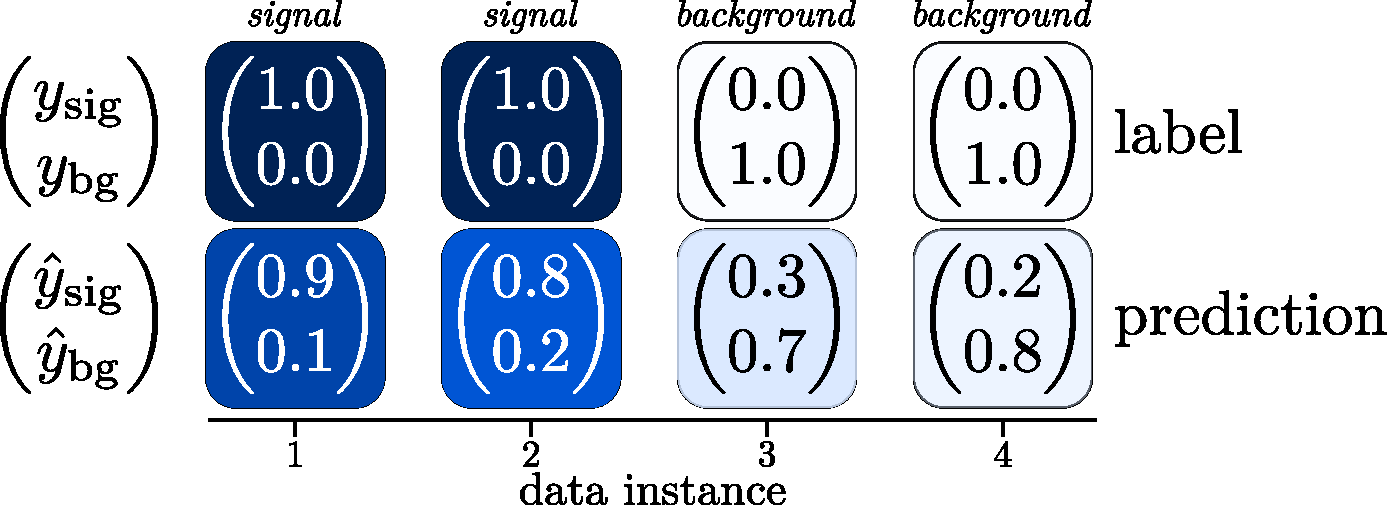
\includegraphics[width=0.85\linewidth]{vector/binary-output.pdf}
    \caption{A representative binary classification output for four hypothetical data instances. While labels $ \y $ give perfect ``one'' or ``zero'' answers, a classifier's actual predictions $ \hat{\y} $ represent a probability for each class in the continuous range $ [0, 1] $.}
    \label{fig:output}
\end{figure}

We now pause to clarify what a binary classifier's output looks like and how to interpret the result. First, we decide on an order in which to quote the possible classes: in this work we will quote signal first, then background. The label, represented by a vector $ \vec{y} $, equals one at the position of the correct class and zero at the position of the incorrect class. In the signal-first convention, a generic label vector reads $ \vec{y} = (y_{\text{sig}}, y_{\text{bg}}) $; the label $ \vec{y} = (1, 0) $ represents signal while $ \vec{y} = (0, 1) $ represents background. Meanwhile, a classifier's prediction, denoted by $ \hat{\y} = (\hat{y}_{\text{sig}}, \hat{y}_{\text{bg}})$, represents the predicted \textit{probabilities} that an event corresponds to either signal or background; these two values should sum to one. Figure \ref{fig:output} summarizes these ideas visually.


% The input layer serves only as a pipeline to pass inputted feature vectors into the network's hidden layers, the output layer produces the classification probability scores for each class, and the hidden layers perform the bulk of the computations producing these classification scores.
\subsection{An Overview of a Fully-Connected Network} \label{ss:fcn-first-look}

\begin{figure}[htb!]
    \centering
    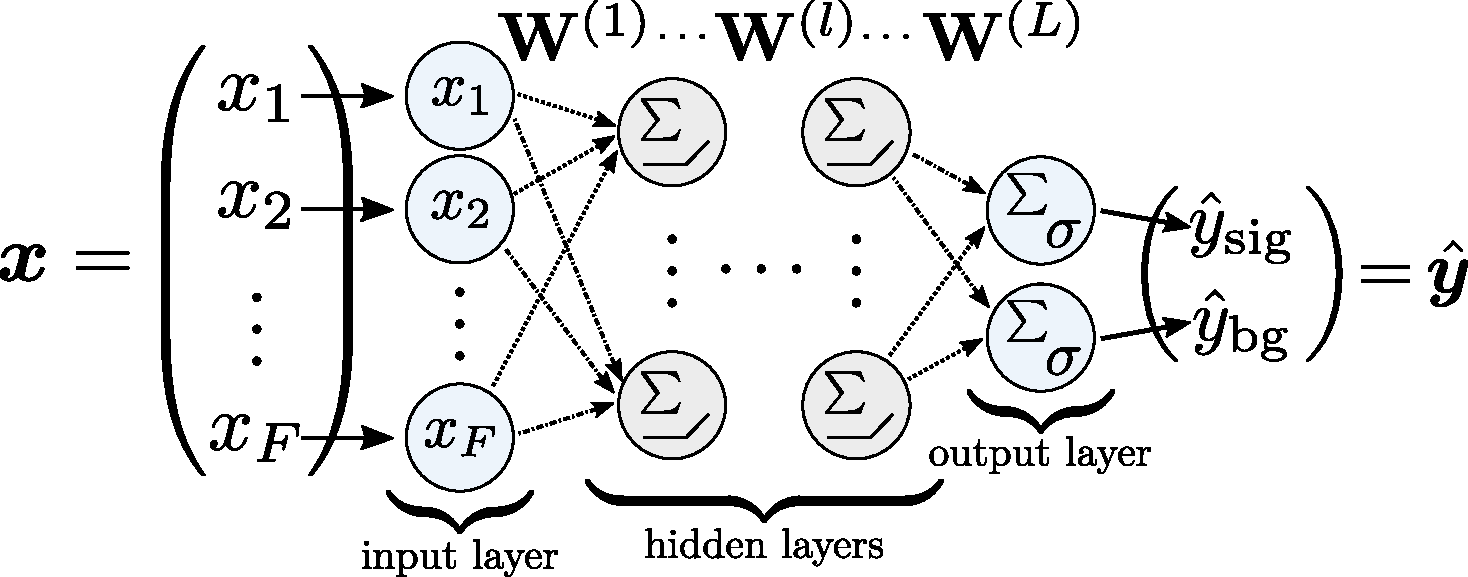
\includegraphics[width=0.95\linewidth]{vector/fcn-architecture.pdf}
    \caption{A fully-connected network's internal architecture; each neuron beyond the input layer connects to \textit{every} neuron in the previous layer. The figure uses the notation from \myhref{s:appendix-fcn}{Appendix \ref{s:appendix-fcn}}. The $ \sum $ (sum) symbol represents the multiply-add neuron operation in Equation \ref{eq:preactivation}, while the hinge and $ \sigma $ symbols represent the ReLU and softmax activation functions, shown in Figure \ref{fig:relu} and Equation \ref{eq:softmax}, respectively.}
    \label{fig:fcn-architecture}
\end{figure}

For better orientation, Figure \ref{fig:fcn-architecture} shows the architecture of a fully-connected neural network. The basic building of a FCN is a \textit{neuron}---represented by the circular nodes in Figure \ref{fig:fcn-architecture}. Neurons are then grouped into one-dimensional stacks to form \textit{layers}. A FCN consists of a single \textit{input layer}, an arbitrary number of \textit{hidden layers}, and a single \textit{output layer}, which outputs the classification scores discussed in Section \ref{ss:output}. 

In this section we build up to a big-picture interpretation of FCN-based classification as the optimization of a vector-valued function, a concept which should be familiar to physicists. That said, before proceeding we first refer interested readers to \myhref{s:appendix-fcn}{Appendix \ref{s:appendix-fcn}}, which thoroughly explains the nuts and bolts of a FCN's internal architecture in the language of the machine-learning literature. However, while it might help demystify the ``black box'' nature of neural networks, this formal treatment can be skipped without loss of continuity.

\subsubsection{The Basic Architecture of a Fully-Connected Network}
A neuron may be viewed as a multi-variable scalar function; in analogy with neuroscience, a neuron's output is called its \textit{activation}, which we will denote by $ a $. When considering the forward flow of information through a neural network, we must consider the following two points. Each hidden layer neuron, which we will also refer to as the ``current neuron'',
\begin{enumerate}[(a)]

    \item \label{item:neuron-input} receives as input the activations $ a^{\text{(prev)}}_{1}, a^{\text{(prev)}}_{2}, \ldots, a^{\text{(prev)}}_{n_{\text{prev}}}  $ of all $ n_{\text{prev}} $ neurons in the previous layer, and

    \item passes its scalar output $ a $ to all neurons in the next layer.

\end{enumerate}
As required by point \ref{item:neuron-input} and visualized in Figure \ref{fig:fcn-architecture}, each hidden-layer neuron has input connections to \textit{every} neuron in the previous layer, hence the name ``fully-connected'' network. The strength of each of these connections is parameterized by a unique scalar \textit{weight} $ w_{j} \in \mathbb{R} $, where $  j = 1, 2, \ldots, n_{\text{prev}} $; in other words, $ w_{j} $ parameterizes the current neuron's connection to the $ j $-th neuron in the previous layer. For compactness, we write the current neuron's weights as the vector
\begin{equation*}
    \w = \big( w_{1}, w_{2}, \ldots, w_{n_{\text{prev}}} \big) \in \mathbb{R}^{n_{\text{prev}}};
\end{equation*}
similarly, the previous layer's activation values are written as the vector
\begin{equation*}
    \a_{\text{prev}} = \Big( a_{1}^{(\text{prev})}, a_{2}^{(\text{prev})}, \ldots, a_{n_{\text{prev}}}^{(\text{prev})} \Big) \in \mathbb{R}^{n_{\text{prev}}}.
\end{equation*}
In addition to its $ n_{\text{prev}} $ weights, the current neuron is parameterized by a single scalar bias $ b $, which serves as an additive constant which can translate the neuron's activation value. 

Next, to understand the current neuron's output, we proceed in two steps:
\begin{enumerate}

    \item First, the input activation values $ a_{j}^{\text{(prev)}} $ from the previous layer's neurons are multiplied with each of their corresponding weights $ w_{j} $, summed, and translated by the current neuron's bias $ b $ to produce a pre-activation value $ z $ given by
    \begin{equation}
        z = w_{1} \cdot a^{\text{prev}}_{1} + \cdots + w_{n} \cdot a^{\text{prev}}_{n} + b = \w \cdot \a_{\text{prev}} + b \in \mathbb{R}. \label{eq:preactivation}
    \end{equation}
    Note that this is just the dot product of the current neuron's weight vector with the previous layer's activation vector, plus the current neuron's bias, i.e. a linear function of the input activations.

    \item Second, the current neuron's pre-activation value $ z $ is passed through a \textit{non-linear} \textit{activation function} $ f_{\text{a}} : \mathbb{R} \to \mathbb{R} $ to produce the scalar activation value
    \begin{equation*}
        a = f_{\text{a}}(z) = f_{\text{a}}\big(\w \cdot \a_{\text{prev}} + b\big) \in \mathbb{R}.
    \end{equation*}

\end{enumerate}

\begin{wrapfigure}{R}{0.36\textwidth}
    \centering
    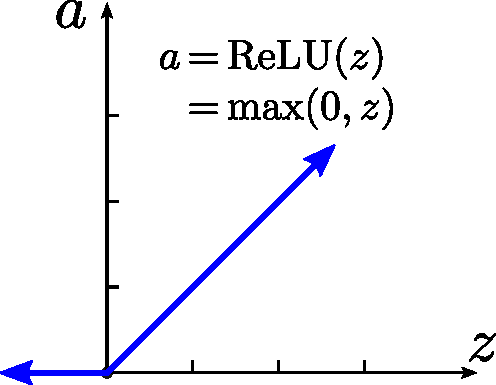
\includegraphics[width=\linewidth]{vector/relu.pdf}
    \caption{The ReLU function}
    \label{fig:relu}
\end{wrapfigure}
Crucially, using \textit{non-linear} activation functions allows the network to form non-linear decision boundaries in the high-dimensional feature space of the inputted feature vectors; these non-linear boundaries enormously improve classification potential. In practice, deep networks predominantly use the rectified linear unit (ReLU) function (Figure \ref{fig:relu}) or one of its variants;\footnote{See Wikipedia's \href{https://en.wikipedia.org/wiki/Activation_function\#Comparison_of_activation_functions}{\underline{list of common activation functions}} for a comprehensive list.} I will use the notation $ f_{\text{a}} $ for generality.

The output layer's activation function is different. At least in classification problems, it is chosen so that the sum of the output layer's activations equals one, giving the interpretation of the output activations as a probability distribution over the possible classes. A common output layer activation function, applicable to an arbitrary number of, say, $ C $ classes, is the softmax function
\begin{equation}
    \sigma (\vec{z})_{i} = \frac{e^{z_{i}}}{\sum_{j = 1}^{C}e^{z_{j}}} \quad \text{for } i = 1, 2, \ldots, C \text{ and } \vec{z} \in \mathbb{R}^{C}. \label{eq:softmax}
\end{equation}

Moving one step up the network hierarchy from a single neuron to an entire layer (which we'll call the ``current layer''), we pack the weight vectors of each of the $ n $ neurons in the current layer column-wise into a weight matrix $ \W $ given by
\begin{equation*}
   \W = \Big( \w_{1} \ \w_{2} \, \cdots \ \w_{n} \Big) = 
    \begin{pmatrix}
        w_{1, 1} & w_{1, 2} & \cdots & w_{1, n}\\
        w_{2, 1} & w_{2, 2} & \cdots & w_{2, n}\\
        \vdots & \vdots & \ddots & \vdots\\
        w_{n_{\text{prev}}, 1} & w_{n_{\text{prev}}, 2} & \cdots & w_{n_{\text{prev}}, n}\\
    \end{pmatrix} \in \mathbb{R}^{n_{\text{prev}}, n},
\end{equation*} 
where the weight $ w_{j, i} $ parameterizes the connection between the $ i $-th neuron in the current layer and the $ j $-th neuron in the previous layer. Similarly, we pack the biases of each neuron in the current layer into a single bias vector
\begin{equation*}
    \b = \big( b_{1}, \, b_{2}, \ldots, \, b_{n} \big)^{\top} \in \mathbb{R}^{n},
\end{equation*} 
where $ b_{i} $ denotes the bias of the $ i $-th neuron in the current layer. Using this matrix formalism, the entire current layer's pre-activation output is compactly written
\begin{equation*}
    \vec{z} = \W^{\top} \a_{\text{prev}} + \b \in \mathbb{R}^{n},
\end{equation*}
while the current layer's activation values read
\begin{equation*}
    \a = f_{\text{a}}(\z) = f_{\text{a}} \Big( \W^{\top} \a_{\text{prev}} + \b\Big) \in \mathbb{R}^{n},
\end{equation*}
where the activation function $ f_{\text{a}} $ is understood to act on the vector $ \z $ element-by-element. The current layer's activation values $ \a $ then serve as input to the next layer, and the cycle repeats. In this way, a feature vector describing a particle collision event propagates through the entire network from input layer to output layer, as shown in Figure \ref{fig:fcn-architecture}. The eventual activation values in the output layer serve as the classification scores discussed in Section \ref{ss:output}, from which we can read off the inputted collision's predicted class.

\subsubsection{FCN Classification as a High-Dimensional Optimization Problem} \label{sss:fcn-interpretation}
We now describe the ``big-picture'' interpretation promised in this section's introduction. A single neuron is a multi-variable scalar-valued function, parameterized by a weight vector $ \w $ and bias $ b $, which takes as input the previous layer's activation $ \a_{\text{prev}} $ and outputs the scalar activation value
\begin{equation*}
    a_{i} = f_{\text{a}} (\w \cdot \a_{\text{prev}} + b) \in \mathbb{R}.
\end{equation*}
Letting $ F $ and $ C $ denote the number of features and classes, respectively, the entire network is a multi-variable vector-valued function $ \vec{h}: \mathbb{R}^{F} \to \mathbb{R}^{C} $, parameterized by the $ L $ weight matrices $ \W^{(l)} $ and bias vectors $ \b^{(l)} $ of each layer. The network takes as input a feature vector $ \x \in \mathbb{R}^{F} $ and produces as output a vector of predicted classification scores $ \hat{\y} \in \mathbb{R}^{C} $, where the component $ \hat{y}_{c} $ gives the probability that the feature vector $ \x $ corresponds to the $ c $-th class, $ c \in \{1, 2, \ldots, C \} $. In this light:
\begin{quote}
    A FCN classification problem is the optimization problem of finding the optimal values $ \W_{\text{opt}}^{(l)} $ and $ \b_{\text{opt}}^{(l)} $ of each layer's weights and biases such that the network's prediction $ \hat{\y} $ for the class of an inputted feature vector $ \x $ gives the best possible approximation to the true result encoded by the label vector $ \vec{y} $.
\end{quote}

\subsubsection{A Brief Look at Optimization} \label{ss:optimization-brief}
Machine learning optimization works by making a neural network's predictions ``less bad'' (rather than, say, improving a positive metric). To proceed, we need a quantitative metric encoding how ``incorrect'' a network's prediction $ \hat{\y} $ is, relative to a known label vector $ \y $. This metric is called \textit{loss}. For a classifier with $ C $ classes, loss is given by a scalar-valued \textit{loss function} $ L : \mathbb{R}^{C} \to \mathbb{R} $, which takes as input a predicted classification score $ \hat{\y} $ and label vector $ \y $, and returns a scalar value $ L $ encoding the difference between $ \hat{\y} $ and $ \y $. For concreteness, an example loss function commonly used for classification problems is the \textit{categorical cross entropy} function
\begin{equation}
    L(\hat{\y}; \y) = - \sum_{c = 1}^{C} y_{c} \ln \hat{y}_{c}. \label{eq:loss-instance}
\end{equation}
For this function, recalling the prediction and label vector structure from \myhref{ss:output}{Section \ref{ss:output}} in which $ y_{c} \in \{0, 1\} $ and $ \hat{y}_{c} \in [0, 1] $, we see that $ L = 0 $ if $ \hat{\y} = \y $, while $ L $ grows increasingly larger as the elements in $ \hat{\y} $ and $ \y $ increasingly differ. 

Put briefly, we optimize the network's weights and biases by minimizing the loss function using standard numerical methods for multi-dimensional minimization problems, but adapted to very large parameter spaces and huge datasets. Interested readers are referred to \myhref{ss:optimization}{Appendix \ref{ss:optimization}} and Chapter 6.5 of Ref. \cite{goodfellow}.

\section{Convolutional Neural Networks}
An end-to-end classification workflow using convolutional neural networks appears in Figure \ref{fig:ccn-in-out}. Our goal in this section, just like in \myhref{s:fcn}{Section \ref{s:fcn}} for FCNs, is to outline what occurs inside the ``Convolutional Neural Network'' box in Figure \ref{fig:ccn-in-out}. As for FCNs, we describe the key ideas here and relegate some technical details to \myhref{s:appendix-cnn}{Appendix \ref{s:appendix-cnn}}, which may be skipped without loss of continuity.  % Fortunately, CNNs and FCNs have much in common, so we are already well on our way. 

\begin{figure}[htb!]
    \centering
    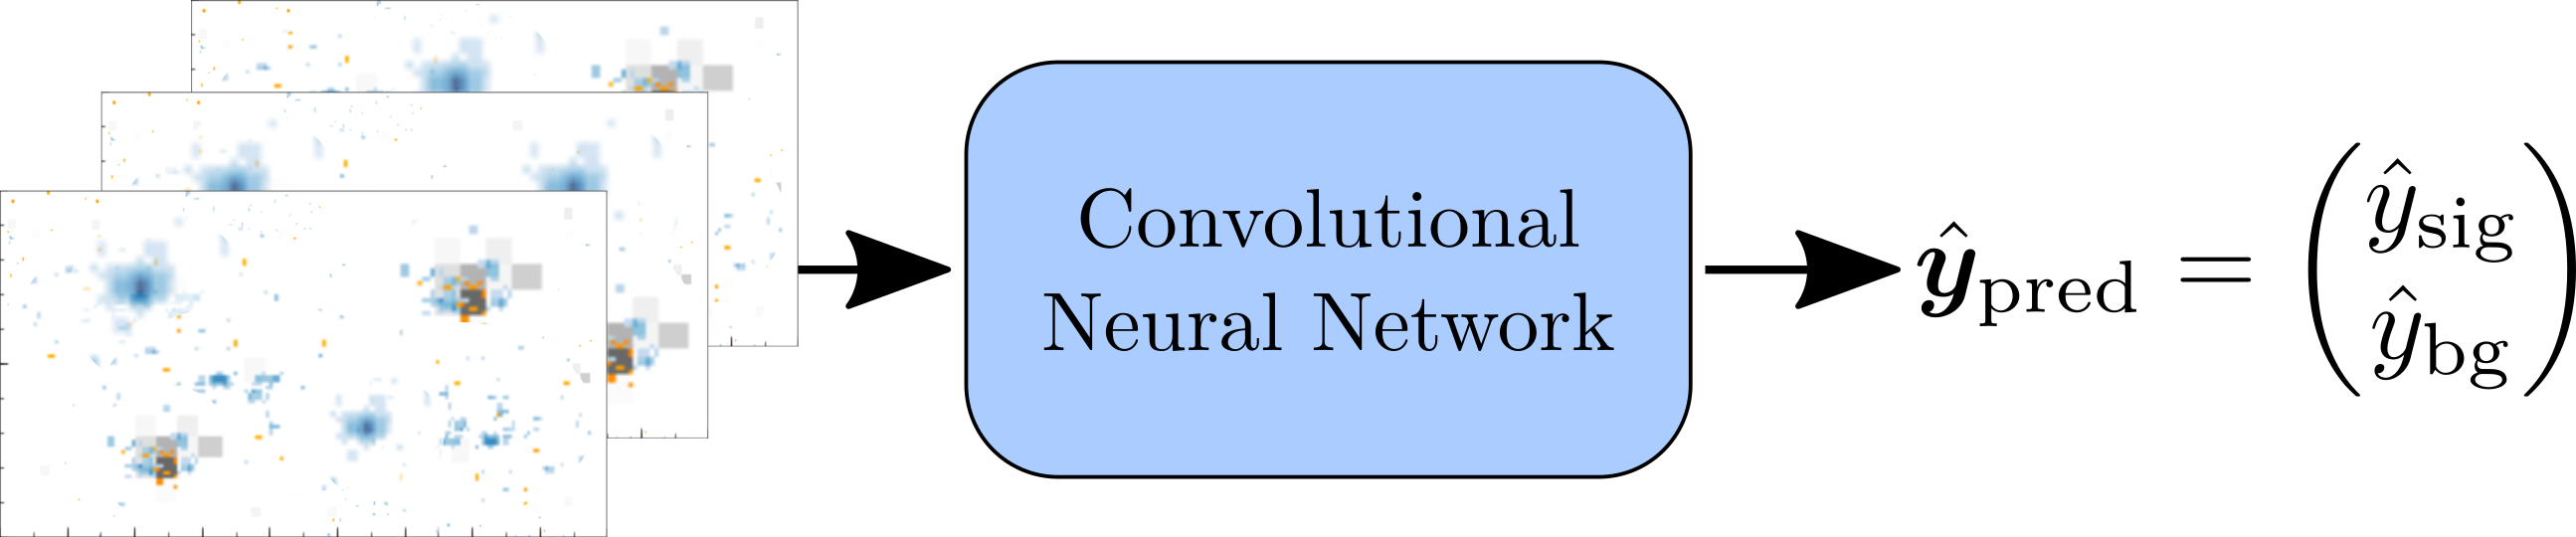
\includegraphics[width=0.9\linewidth]{raster/raster-svg/cnn-in-out.png}
    \caption{The binary classification process using a CNN. Instead of using reconstructed kinematic quantities, the classifier works directly with image-based detector data (cf. Figure \ref{fig:fcn-in-out}).}
    \label{fig:ccn-in-out}
\end{figure}

Suppose, as shown schematically in Figure \ref{fig:ccn-in-out}, that we have a set of image-based, low-level detector data of the same form as Figure \ref{fig:data-raw-ecal}; these images will serve as input to our CNN. Let's begin by analyzing the properties of our input data. Paraphrasing from the excellent explanation in Ref. \cite{cnn-guide}, our image-based detector data:
\begin{enumerate}[(a)]

    \item is stored as multi-dimensional arrays,

    \item has one axis---the detector channel---used to access different views of a collision event from the three CMS subdetectors (Tracker, ECAL, and HCAL), and % in principle, order could matter here as well, no?

    \item \label{item:cnn-order} has two spatial axes---for the coordinates $ \varphi $ and $ \eta $---with well-defined spatial structure in which ordering matters.

\end{enumerate}
Point \ref{item:cnn-order} is especially important. In an image such as Figure \ref{fig:data-raw-ecal}, the relative positions and intensities of the pixels encode a wealth of relevant physical information about particle trajectory and energy, as discussed in \myhref{ss:quantify-decay}{Sections \ref{ss:quantify-decay}} and \ref{ss:three-methods}. Even if you forget everything else about CNNs, you should remember this:
\begin{quote}
    Convolutional neural networks are designed to \textit{preserve and leverage the information encoded in an input image's spatial structure} (in a way that FCNs, which are limited to one-dimensional vector inputs, cannot).
\end{quote}
We thus need a novel, space-preserving way for convolutional networks to interact with their input images. Instead of flattening the input into a large vector, we might imagine ``scanning'' the two-dimensional image with a small, also two-dimensional ``filter'', which moves across the image and builds up a map of distinguishing features, such as bright spots, curves, or edges. This is the essence of a \textit{discrete convolution}, the core (and namesake) operation of CNNs and the subject of the next section.

\subsection{Discrete Convolution} \label{ss:discrete-conv}

A discrete convolution involves two multidimensional objects---an input image and a \textit{kernel} or \textit{filter}. The kernel is a pixel-like grid like the input image, but always smaller in height and width. Each kernel pixel is assigned a scalar \textit{weight}, and the kernel as a whole a single scalar \textit{bias}; these kernel weights and biases are a CNN's tunable parameters, and replace the neuron weights and biases in a FCN \cite{homl, goodfellow}.

During discrete convolution,\footnote{Formally, the operation commonly called discrete convolution is actually cross-correlation; true convolution employs a kernel whose elements are reflected across the spatial axes. This technicality is irrelevant in practice; see Chapter 9.1 of Ref. \cite{goodfellow} for a more thorough discussion.} the kernel slides across the input image from left to right and top to bottom, and at each possible position the kernel and input elements are multiplied element-wise and summed to produce a single scalar value. The set of these scalar products at each possible kernel position within the input image produces the output, called an \textit{output feature map}, again an image-like pixel grid. This is awkward to explain in words but straightforward visually---hence Figure \ref{fig:conv-single-channel}. Importantly, a discrete convolution's output has the same dimensional form as its input, and can thus be used as the \textit{input feature map} to another convolutional layer. 

\begin{figure}[htb!]
    \centering
    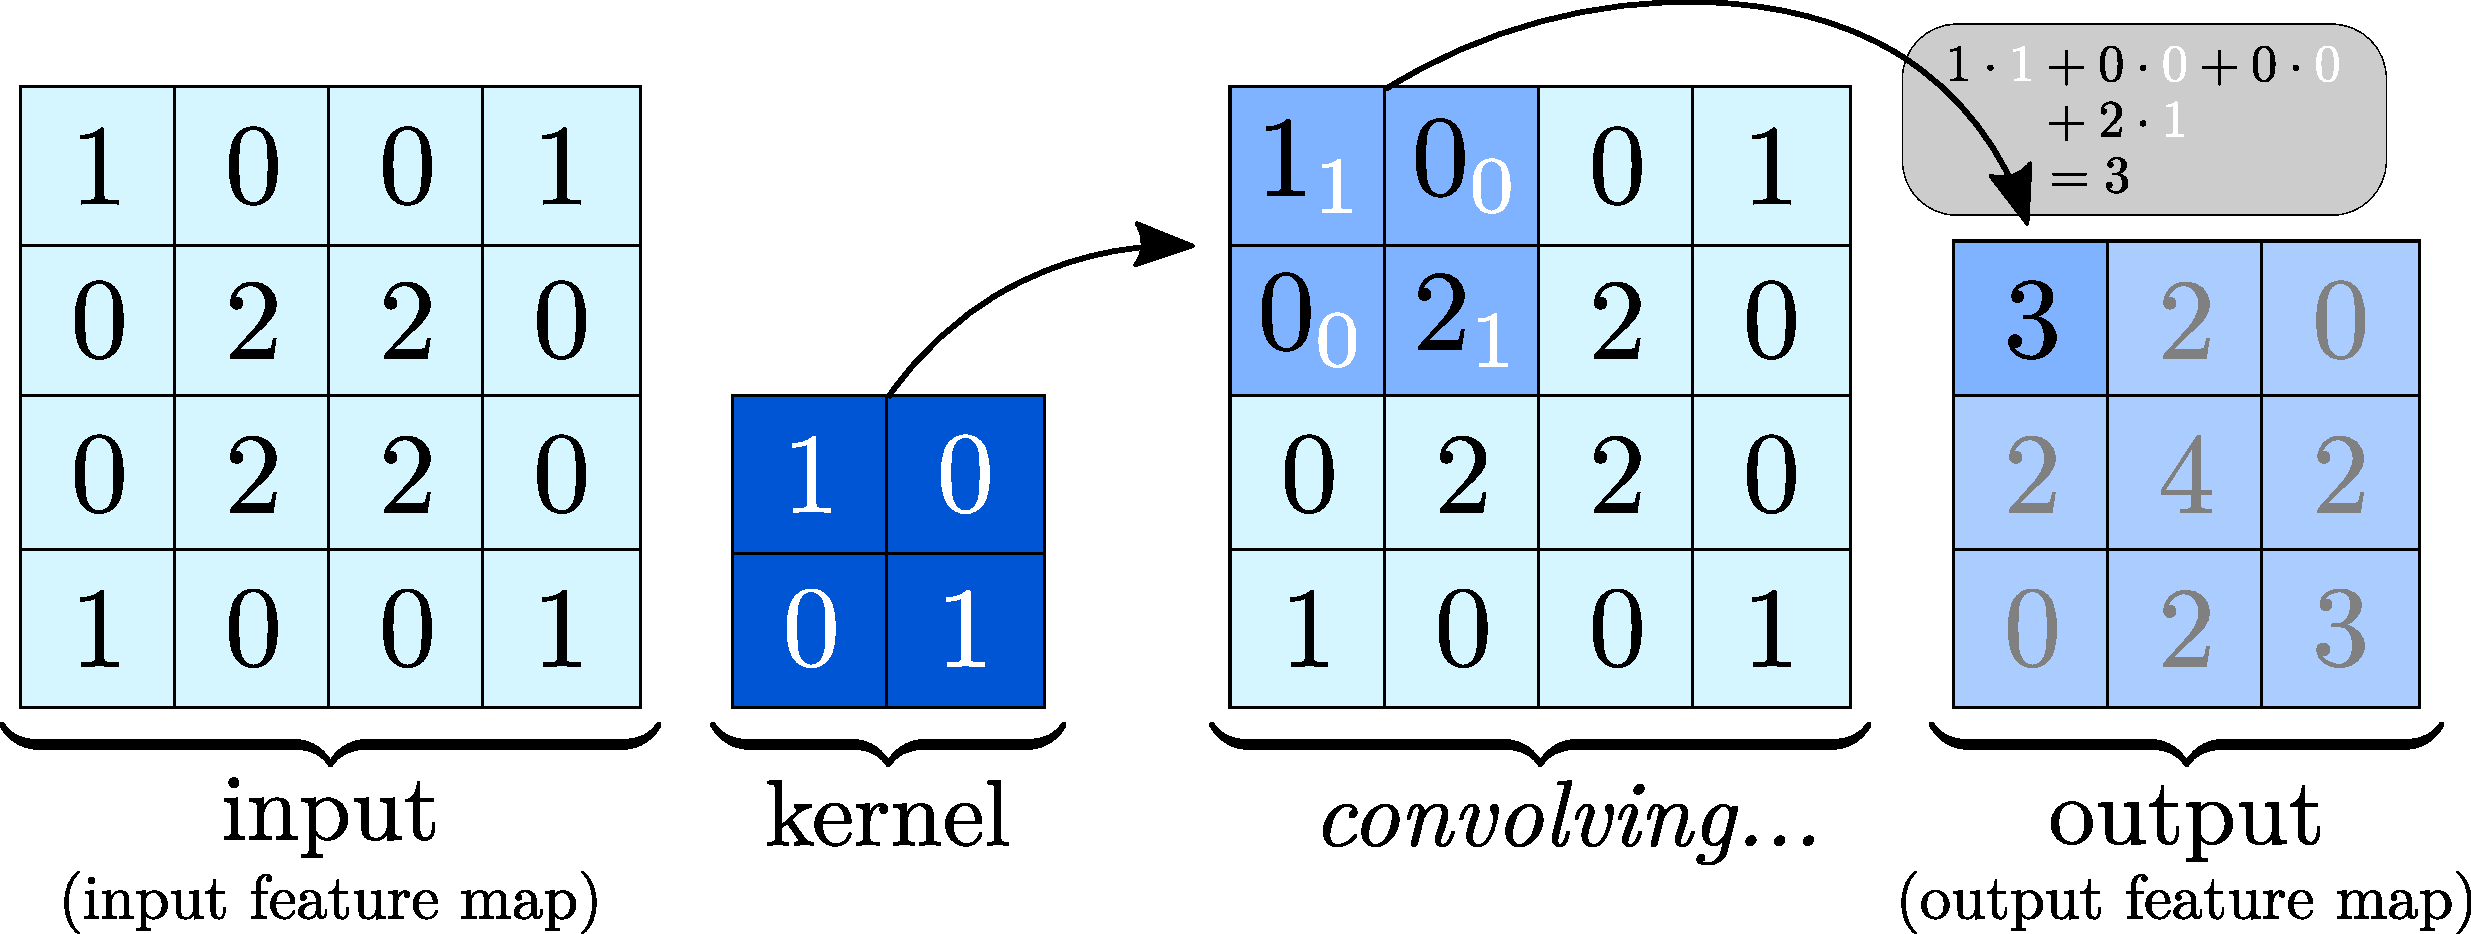
\includegraphics[width=0.8\linewidth]{vector/conv-single-channel.pdf}
    \vspace{-2mm}
    \caption{A toy example of a discrete convolution. The kernel is placed at each possible position in the input, and the kernel and input are multiplied element-wise and summed to form the output values. The kernel's bias is omitted for conciseness.}
    \label{fig:conv-single-channel}
\end{figure}

In practice, images are three-dimensional---they contain multiple channels, such as the three subdetector channels in our CMS detector data or the three color channels in RGB images. In this case the convolutional kernel is also three dimensional, with a separate kernel channel for each image channel, as shown in Figure \ref{fig:conv-multi-channel}. After convolution, a kernel's outputs are summed across the channel axis to produce a scalar value for each spatial position of the kernel within the input image. The end result is again a two-dimensional output feature map, as in Figure \ref{fig:conv-multi-channel}. Mathematical relationships between kernel, input, and output size are given in \myhref{ss:conv-arithmetic}{Appendix \ref{ss:conv-arithmetic}}

\begin{figure}[htb!]
    \centering
    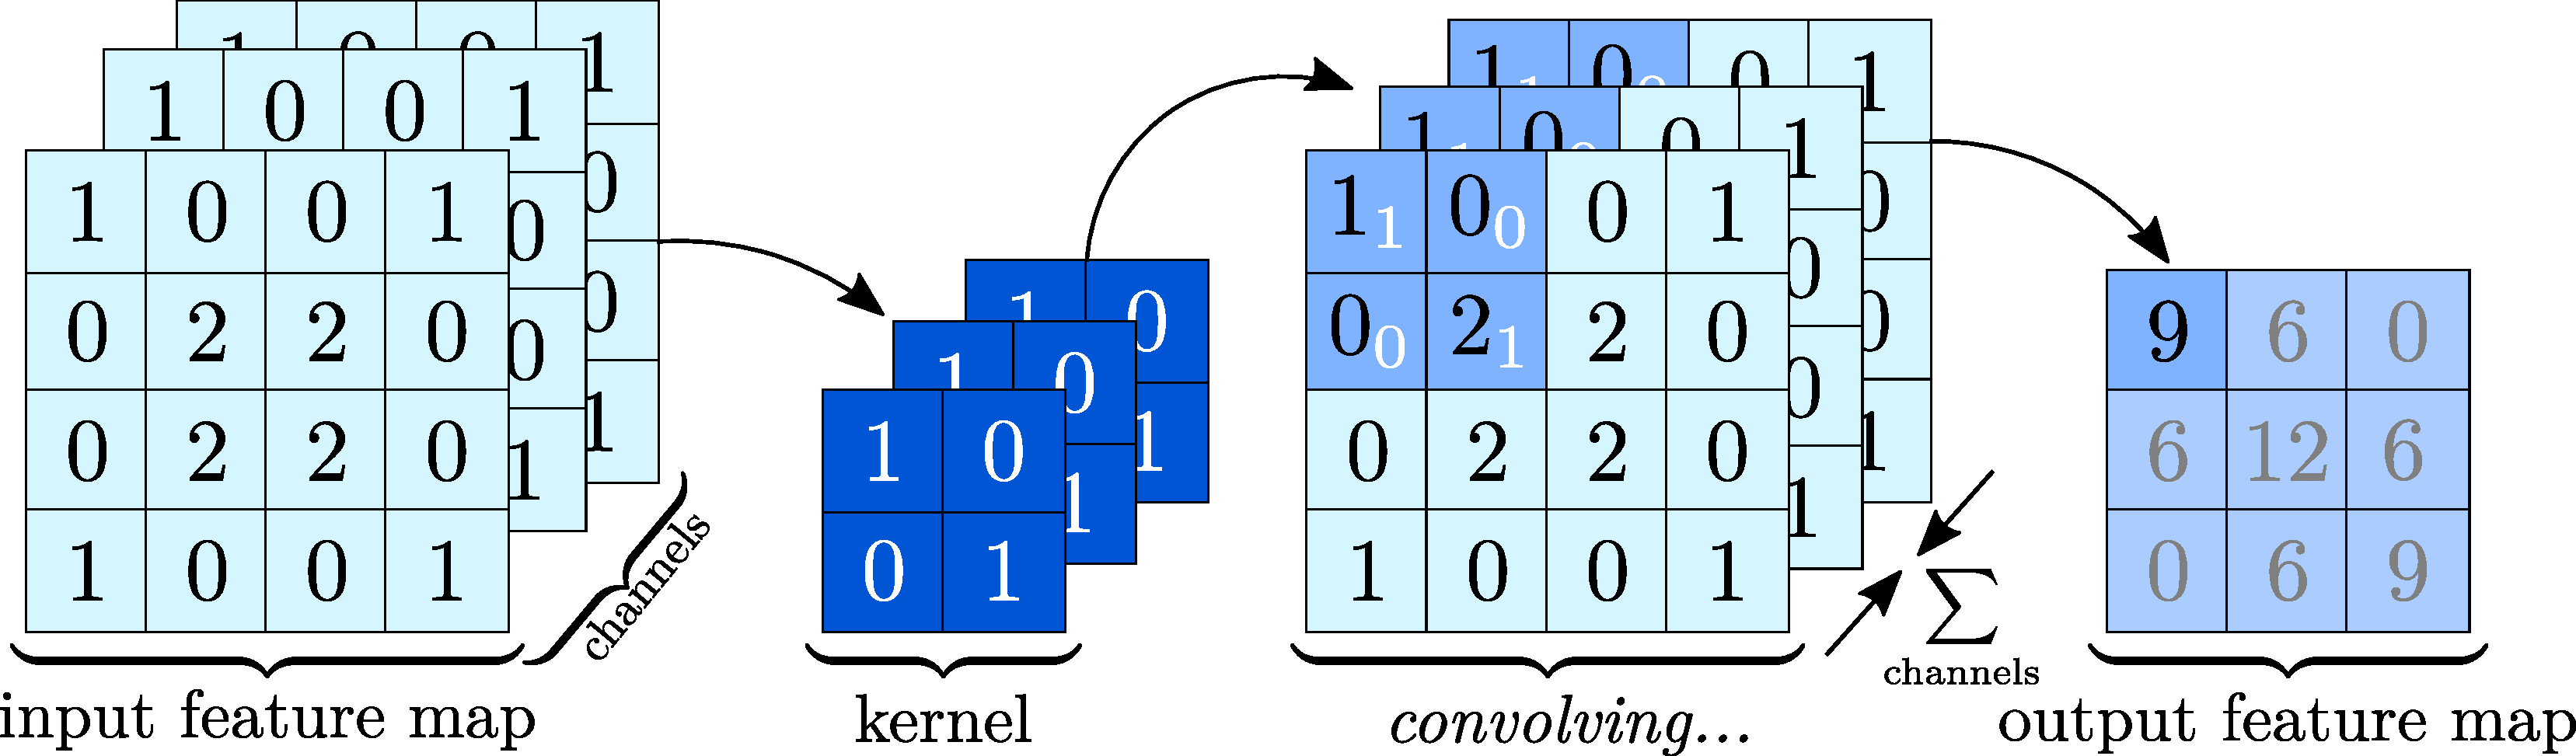
\includegraphics[width=0.9\linewidth]{vector/conv-multi-channel.pdf}
    \caption{Discrete convolution with multiple channels in the input; cf. Figure \ref{fig:conv-single-channel}. The convolutions from each channel are summed across the channel axis to produce a single-channel output. In practice, of course, the input and kernel would have different values in each channel. The kernels' biases are omitted for conciseness.}
    \label{fig:conv-multi-channel}
\end{figure}

In practice, as shown schematically in Figure \ref{fig:cnn-architecture}, CNNs also convolve a single input feature map with \textit{multiple} kernels---just like FCNs employ multiple neurons in each fully-connected layer. Each kernel captures different feature information (edges, curves, contrasting colors...) describing the input image, so using more kernels improves potential classification power. In this case, a convolutional layer's output is three dimensional (with as many channels as the number of kernels used for convolution) and serves as the multi-channel input to a subsequent convolutional layer.

\subsection{Pooling}

\begin{figure}[htb!]
    \centering
    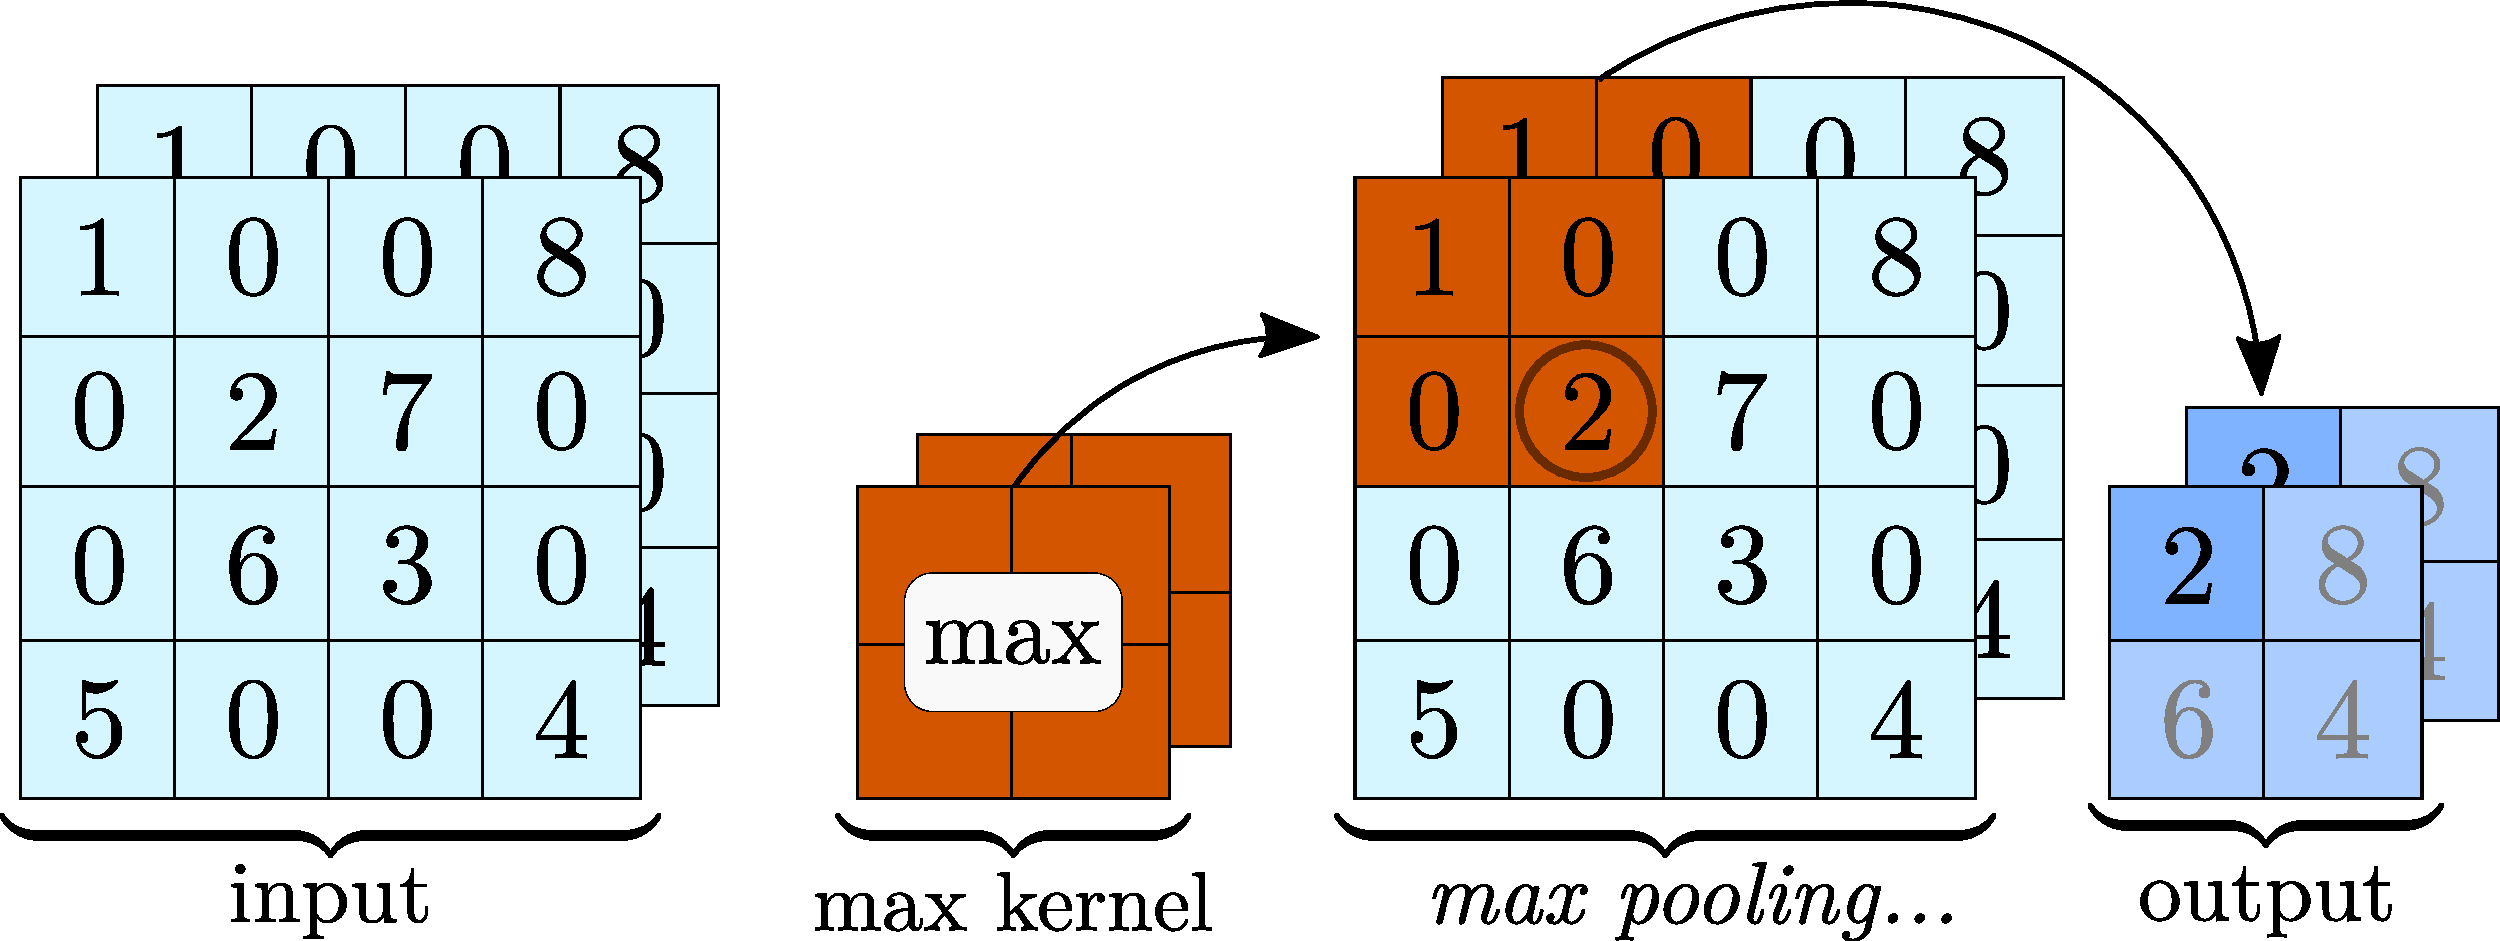
\includegraphics[width=0.8\linewidth]{vector/pooling.pdf}
    \vspace{-2mm}
    \caption{The max pooling operation. The kernel moves in non-overlapping patches across the input and outputs the maximum pixel value at each patch. Note that, unlike discrete convolution (Figure \ref{fig:conv-multi-channel}) pooling preserves the channel dimension.}
    \label{fig:pooling}
\end{figure}
Convolutional networks also employ a second, simpler operation called \textit{pooling}. Pooling serves two purposes; these are to:
\begin{itemize}

    \item make the CNN's output invariant to local translations of the input image, and

    \item spatially downsample an input without introducing new learnable parameters. 

\end{itemize}
Pooling involves a pooling kernel, which is analogous to the convolutional kernel, but simpler. Most commonly, the pooling kernel slides across an input feature map's spatial dimensions in non-overlapping patches, and outputs the maximum pixel value at each kernel position. Pooling preserves channel dimensions, so a pooling stage's output always has the same number of channels as the input, as shown in Figure \ref{fig:pooling}. 

In principle, the pooling kernel could also move across overlapping or arbitrarily-strided patches, and output, say, the average pixel value (\textit{average pooling}) instead of the maximum (\textit{max pooling}). However, max pooling with non-overlapping strides appears most commonly in modern CNNs \cite{homl}. 


% Pooling acts only along spatial dimensions, and preserves the channel dimension. For any input and pooling kernel dimensions $ I_{j} $, $ K_{j}^{(\text{p})} $ and any kernel stride $ s_{j} $, the output size of a pooling layer along the axis $ j $ is
% \begin{equation}
%     O_{j}^{(\text{p})} = \floor*{\frac{I_{j} - K_{j}^{(\text{p})}}{s_{j}}} + 1; \label{eq:cnn-O-pool}
% \end{equation}
% this is simply Equation \ref{eq:cnn-O-conv} with $ p_{j} = 0 $, since pooling does not involve zero padding.

% Essentially: pooling splits the input image into (generally) non-overlapping patches along the spatial dimensions and outputs the maximum pixel value of each patch.

\subsection{The Basic Architecture of a Convolutional Network} \label{ss:cnn-architecture}

\begin{figure}[htb!]
    \centering
    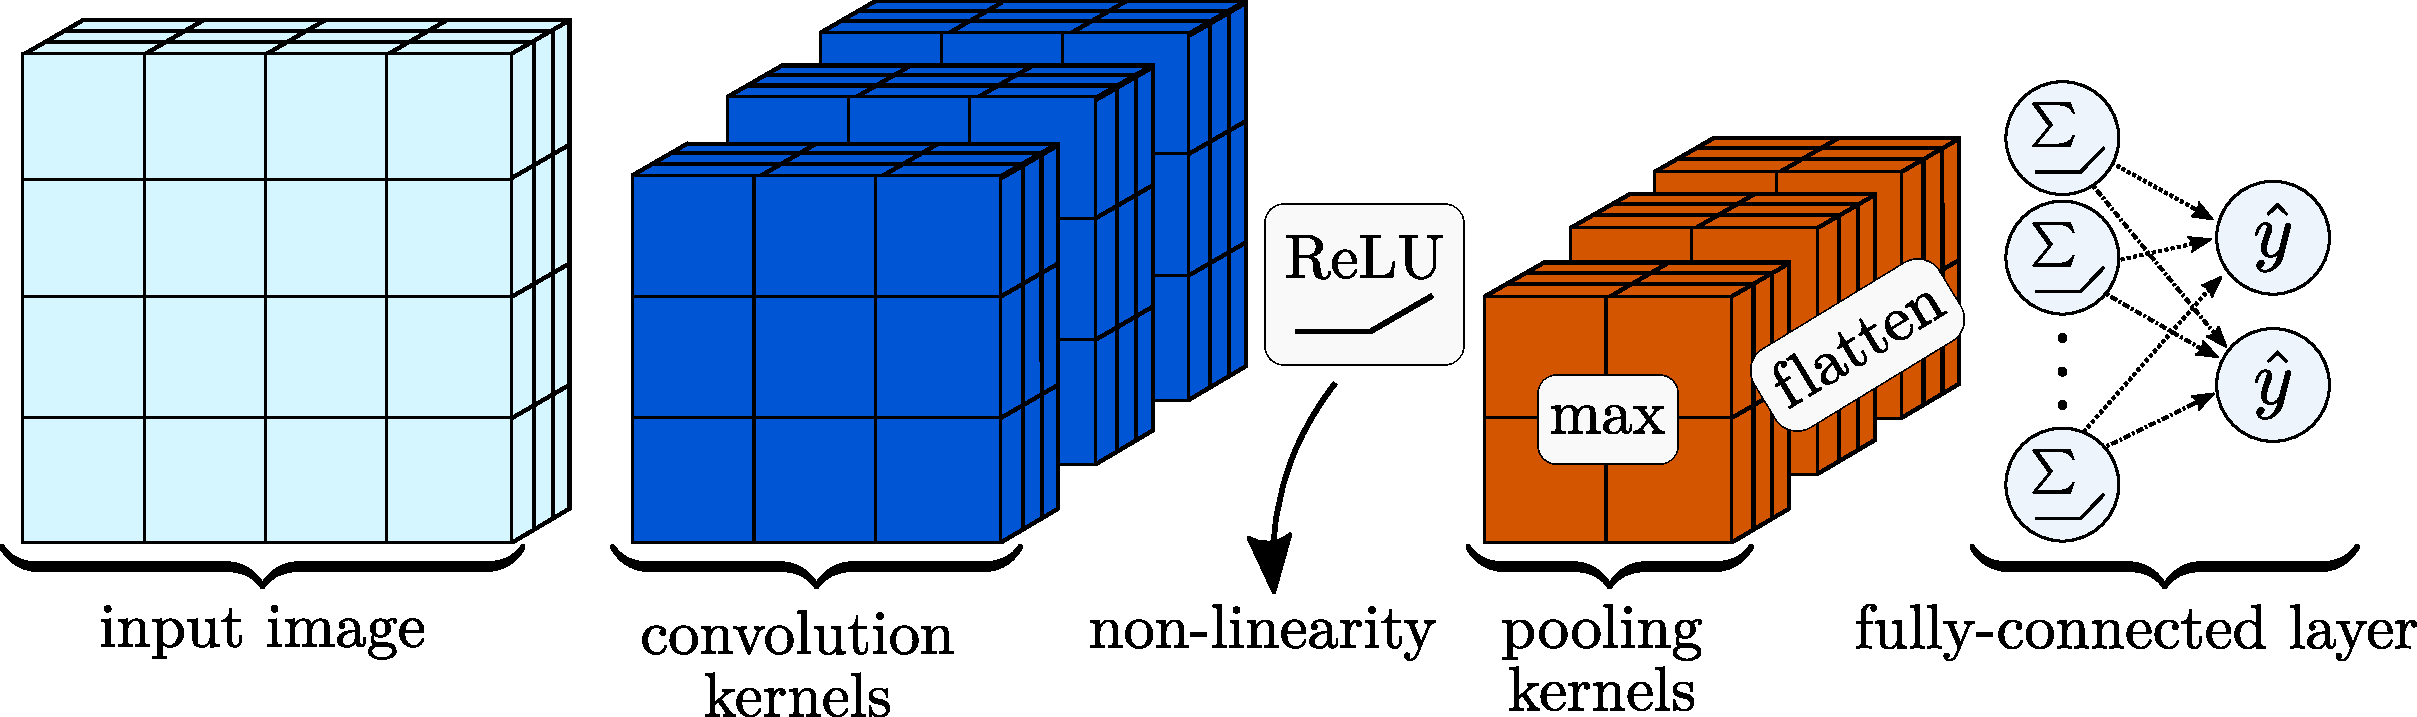
\includegraphics[width=0.95\linewidth]{vector/cnn-architecture.pdf}
    \caption{The important stages of a convolutional network in their typical sequence.}
    \label{fig:cnn-architecture}
\end{figure}

Figure \ref{fig:cnn-architecture} shows the typical sequence of operations in a CNN: an input image is processed by multiple kernels in a convolutional layer, passed element-wise through a non-linearity (most commonly a ReLU), and downsampled in a pooling layer.\footnote{In practice, a convolutional stage's outputs are usually also normalized to zero mean and unit variance in a \textit{normalization layer}, which is empirically found to improve training performance \cite{homl}.} The process then repeats, with one stage's output feature map used as the input to the next stage. Finally, the output of the last pooling layer is flattened into a one-dimensional vector and passed through a single fully-connected layer to produce classification scores in an identical format as already seen for FCNs in \myhref{ss:output}{Section \ref{ss:output}}.

For CNNs, we tune the convolutional kernels' weights and biases instead of the neuron weights and biases in FCNs. The general principles of loss, optimization and backpropagation through computational graphs discussed in \myhref{ss:optimization}{Appendix \ref{ss:optimization}} in the context of FCNs still apply to CNNs, and we will not repeat them here.

% \begin{itemize}

%     % \item Define input images with shape $ C_{\text{in}}, I_{\text{w}}, I_{\text{h}} $. Define input layer. This is a convolutional layer. 

%     % Define an arbitrary number of filters to use in the input layer. Each filter has dimensions $ (C_{\text{in}}, K_{\text{w}}, I_{\text{h}}) $. Use $ C_{\text{out}} $ such filters. Perform discrete convolutions of an input image with each filter as described in \myhref{ss:discrete-conv}{Section \ref{ss:discrete-conv}} and shown Figure \ref{fig:conv-multi-channel}. The result is an output with shape $ (C_{\text{out}}, O_{\text{w}}, O_{\text{h}}) $, where $ O_{\text{w}} $ and $ O_{\text{h}} $ as described in \myhref{ss:conv-arithmetic}{Section \ref{ss:conv-arithmetic}}.

% \end{itemize}

\section{End-to-End Classification in Practice}
\subsection{A Case Study in End-to-End Classification}
For concreteness, we now summarize an actual study involving end-to-end classification: the work of Andrews et al. in Ref. \cite{andrews-higgs}. This study uses convolutional neural networks to distinguish diphoton Higgs boson decays from two similar background events using simulated CMS data. The study considers the following three processes: (i) gluon fusion Higgs production to diphoton decay  $ gg \to H^{0} \to \gamma \gamma $ (signal); (ii) quark-antiquark annihilation to diphoton decay $ q \bar{q} \to \gamma \gamma $ (background); and quark-antiquark annihilation to photon+jet decay $ q \bar{q} \to \gamma j $ (background). Representative Feynman diagrams for the signal and diphoton background process appear in Figure \ref{fig:feynman-signal-bg}, while the relevant datasets may be found in Refs. \cite{data-bg-diphoton}, \cite{data-bg-jet}, and \cite{data-signal}.
 


\begin{figure}[htb!]
    \centering
    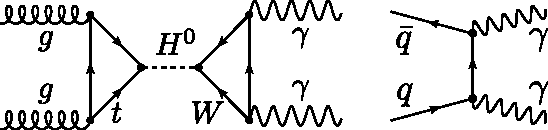
\includegraphics[width=0.8\linewidth]{vector/feynman-signal-bg.pdf}
    \caption{Representative Feynman diagrams showing the signal (left) and diphoton background (right) processes in Andrews' study. For the purposes of this work, it suffices to note that both processes share identical $ \gamma \gamma $ backgrounds.}
    \label{fig:feynman-signal-bg}
\end{figure}

The two background processes are chosen specifically to represent two common challenges in high-energy physics particle classification. These are:
\begin{enumerate}[(a)]

    \item \textit{irreducible backgrounds}---the diphoton background has identical decay products to the signal process, as shown in Figure \ref{fig:feynman-signal-bg}---and % The background must be differentiated from signal on kinematic grounds.

    \item \textit{unresolved decay products}---for reasons irrelevant to this work,\footnote{For the sake of completeness, the jet is electromagnetically enriched to deposit its energy primarily in the ECAL via a neutral meson decaying to two merged photons \cite{andrews-higgs, data-bg-jet}.} the jet in the $ \gamma j $ background appears in the ECAL detector as a single, photon-like cluster, so the $ \gamma j $ decay signature appears similar to its $ \gamma \gamma $ counterpart.

\end{enumerate}
The study uses a 15-layer variant of a common CNN architecture called a \textit{residual network} (ResNet), which employs a structure called a ``residual block'', in which inputted feature maps are allowed to bypass convolutional layers; interested readers are referred to Chapter 14, page 457 of Ref. \cite{homl}. As input, the CNN classifier accepts the same image-like data shown in Figure \ref{fig:data-raw-ecal}, and outputs \textit{three} classification scores $ \hat{y}_{\text{sig}} $, $ \hat{y}_{\text{bg}_{\gamma\gamma}} $, and $ \hat{y}_{\text{bg}_{\gamma j}} $, representing the predicted probabilities for each of the three processes considered in the study. For reference, the study also classifies the same datasets using a kinematics-based FCN classifier, discussed in \myhref{s:fcn}{Section \ref{s:fcn}}. This FCN is trained on the transverse momenta, pseudorapidities, and azimuthal angles of the decay particles, and the results are compared to those obtained by the CNN. 

\subsubsection{Discussion of Results}

\begin{wrapfigure}{R}{0.5\textwidth}
    \centering
    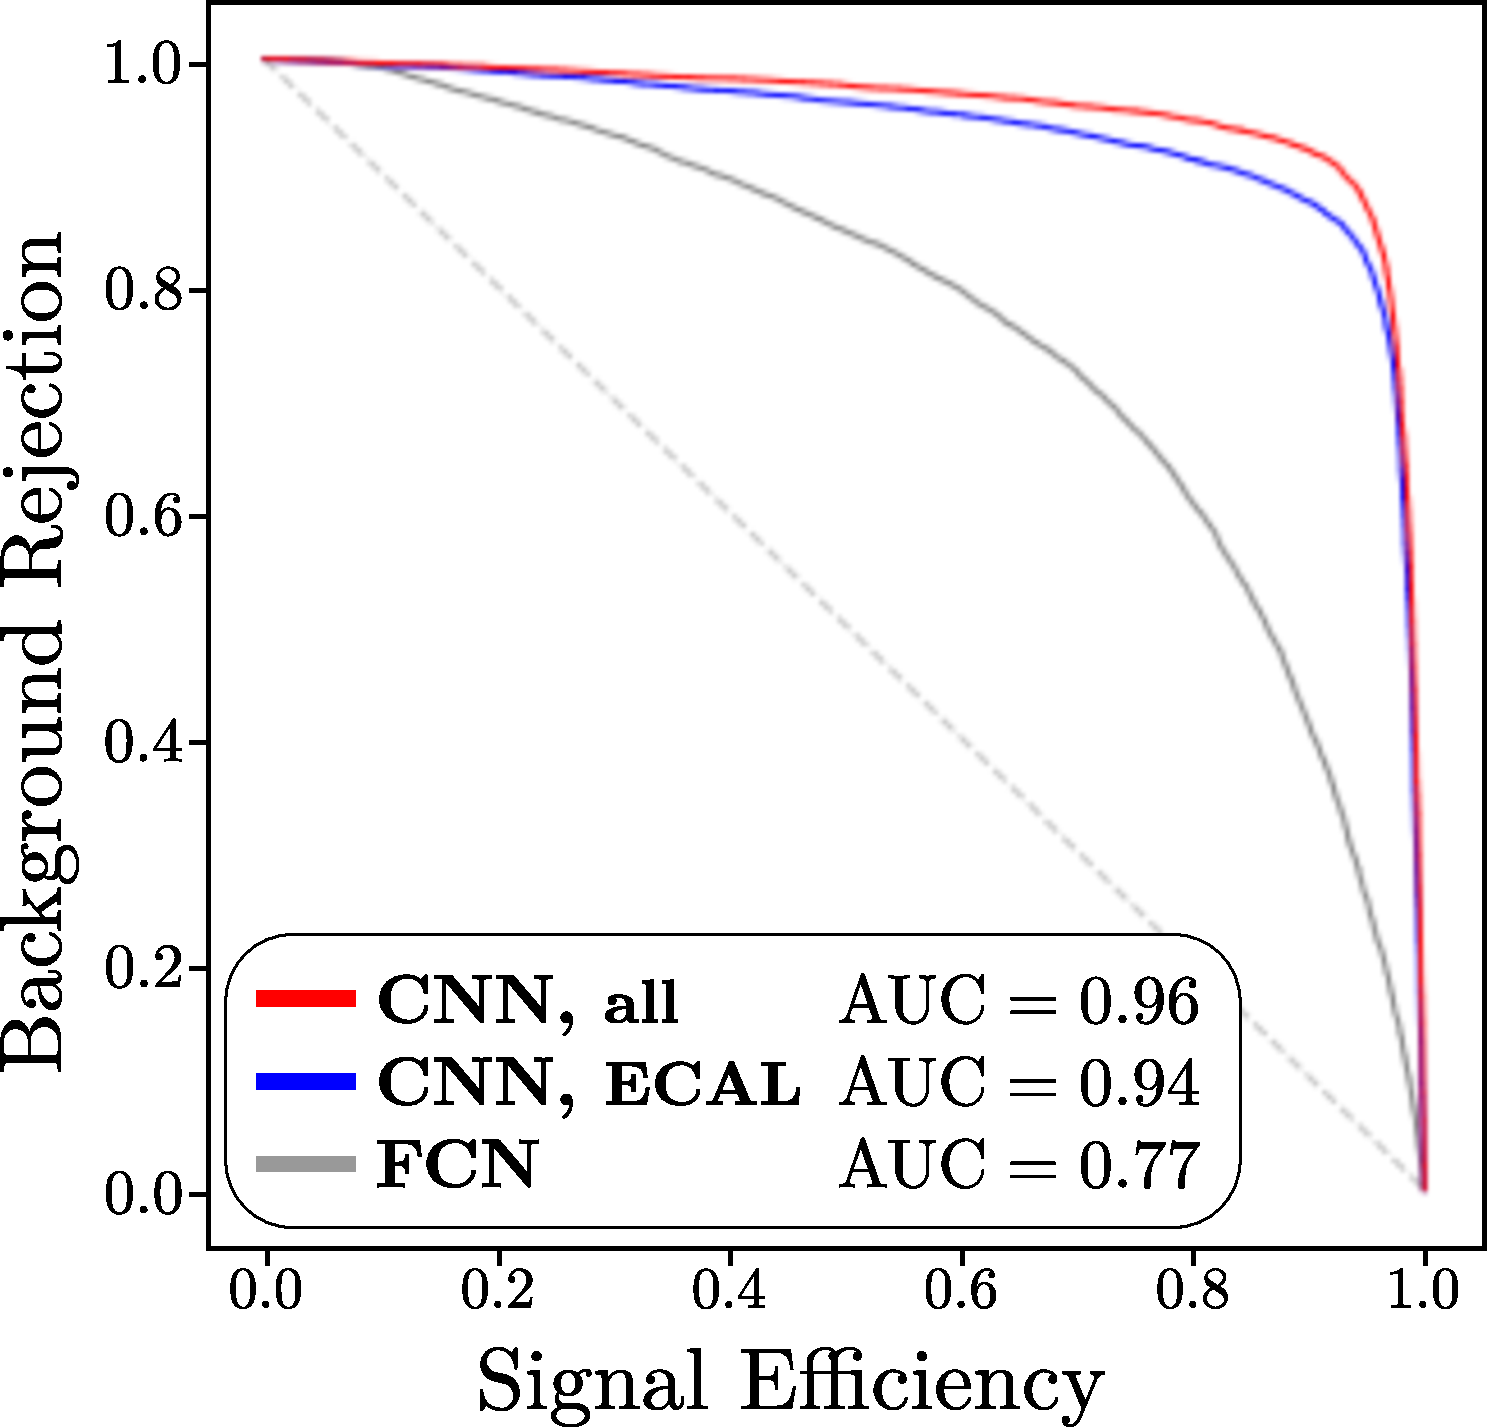
\includegraphics[width=\linewidth]{raster/raster-svg/roc.pdf}
    \vspace{-8mm}
    \null \hspace{10mm}\caption{An ROC curve showing the results for a kinematic-based FCN (gray) and two end-to-end CNN (blue and red) classifiers for distinguishing $ H \to \gamma \gamma $ signal and $ \gamma j $ background. Adapted from \cite{andrews-higgs}.}
    \label{fig:andrews-roc}
\end{wrapfigure}

We now briefly examine one of the study's more interesting results. Namely, we compare the performance of the FCN and the two CNN classifiers when distinguishing $ H \to \gamma \gamma $ signal and $ q \bar{q} \to \gamma j $ background events; one CNN is trained only with ECAL data (\textbf{CNN, \small{ECAL}}) and one with Tracker, ECAL and HCAL data (\textbf{CNN, \small{all}}). The classifications results are shown in Figure \ref{fig:andrews-roc} with a receiver-operating characteristic (ROC) curve, which shows a classifier's background rejection as a function of classification efficiency. From Figure \ref{fig:andrews-roc}, we immediately see that, in this particular case, the CNN classifiers substantially outperform their FCN counterpart.

To interpret this discrepancy, it helps to remember what the relevant detector data actually looks like; recall that a representative $ \gamma j $ background event appears in Figure \ref{fig:data-raw-ecal}. A human, equipped with the power of vision, can immediately distinguish the photon and jet in Figure \ref{fig:data-raw-ecal}. Aside from the obvious fact that the hadronic jet carries Tracker and HCAL hits, we also notice subtle differences in shower distribution---the photon's hits are concentrated and circular, while the jet's are more dispersed and dragged out elliptically along the $ \varphi $ axis. However, we might struggle to give an answer if the only information we received were the momentum and $ (\varphi, \eta) $ coordinates of the two events. But that is precisely the information seen by a kinematic-based FCN! A CNN, meanwhile, is designed to preserve and learn from the entire image's spatial structure; hence the improved performance seen in Figure \ref{fig:andrews-roc}. In other words, CNN classifiers using low-level detector data show promise for distinguishing between processes with subtle differences in shower distribution, and thus offer a powerful classification tool for high-energy physicists in the search for new physical processes.

\subsection{Concluding Thoughts}
Using raw detector data, without further processing, preserves the maximum available physical information about a particle collision event. Since convolutional networks are better suited to learning from the spatial information encoded in raw detector data than fully-connected networks, CNNs and the end-to-end classifiers employing them show a clear advantage over kinematic feature-based classifiers for processes distinguished by subtle difference in particle shower distributions. 

The benefits of end-to-end classification are numerous. Aside from their greatest benefit---preserving and learning from spatial information---end-to-end workflows provide a general, widely applicable framework to particle classification. Because of their low-level inputs, end-to-end classifiers mitigate our reliance on particle flow reconstruction of kinematic features, and potentially eliminate completely the need for manual engineering of high-level features on a case-by-case basis. 

Additionally, although not discussed in this work, using traditional FCN classifiers with processes involving many (or a variable number of) decay products poses a considerable technical challenge \cite{andrews-higgs}. For CNNs such issues are avoided altogether---one simply inputs raw detector data and training labels, and the CNN develops its classification power from the spatial distribution of the particle showers. As such, CNN-based end-to-end classifiers offer a promising tool for analyzing the increasingly complex processes and weaker signals involved in modern particle physics and the search for physics beyond the Standard Model.


\newpage
\appendix
\section{A Technical Discussion of FCNs} \label{s:appendix-fcn}
We begin by introducing the notation\footnote{Note that some of the notation used in this work is not standard, but chosen on pedagogical grounds for better semantics (e.g. $ {\color{myMaroon} l} $ to index {\color{myMaroon} l}ayers, $ {\color{myMaroon} c} $ to index {\color{myMaroon} c}lasses, $ {\color{myMaroon} a} $ for {\color{myMaroon} a}ctivation value, etc...).} needed to describe a FCN:
\begin{itemize}

    \item Let $ F $ denote the number of features and $ C $ the number of classes. A binary classifier with two classes has $ C = 2 $, but we use $ C $ for generality.

    \item Let $ L $ denote the number of hidden layers (so that the network has $ L + 1 $ layers when including the input layer).

    \item Let $ l = 0, 1, 2, ..., L $ index the layers, with $ l = 0 $ the input layer and $ l = L $ the output layer.

    \item Let $ n_{l} $ be the number of neurons in layer $ l $, and let $ i $, where $ i = 1, \ldots, n_{l} $, index the neurons in each layer. A neuron's position in the network is uniquely defined by the layer $ l $ and index $ i $.

    % The number of of neurons in the input layer is $ n_{0} = F $.
    % The number of neurons in the output layer is $ n_{L} = C $.

\end{itemize}
% \textit{Note}: The following two sections contain a lot of information. From personal experience, keeping track of the relationships between weights and biases across network layers may be overwhelming to the unfamiliar reader on a first attempt. Unfortunately, I know of no way around this if we wish to meaningfully understand a neural network beyond mere hand-waving. To make things easier, I have paid utmost care to consistent and semantically meaningful notation, while a more intuitive ``big-picture'' interpretation of a neural network follows in \myhref{ss:fcn-interpretation}{Section \ref{ss:fcn-interpretation}}.

\subsection{Weights and Biases}
\small{\textit{The purpose of the weights and biases appears immediately below in} \myhref{ss:response-activation}{Appendix \ref{ss:response-activation}}.}

\vspace{2mm}
Consider an arbitrary $ i $-th neuron in the network's $ l $-th layer, and, for better semantics, let $ n_{\text{prev}} \equiv n_{l - 1} $ denote the number of neurons in the previous layer. This generic $ l $-th layer neuron is assigned:
\begin{enumerate}

    \item A total of $ n_{\text{prev}} $ scalar \textit{weights} $ w_{j,i}^{(l)} \in \mathbb{R} $, contained in a weight vector
    \begin{equation}
        \w_{i}^{(l)} = \Big(w_{1, i}^{(l)}, \, w_{2, i}^{(l)}, \ldots, \, w_{n_{\text{prev}}, i}^{(l)}\Big)^{\top} \in \mathbb{R}^{n_{\text{prev}}}. \label{eq:weight-vector}
    \end{equation}
    Each $ l $-th layer neuron connects to all $ n_{\text{prev}} $ neurons in the previous layer, and the $ n_{\text{prev}} $ weights parameterize these connections (see Figure \ref{fig:fcn-architecture}). Going forward, I will drop the $ {}^{(l)} $ superscript from individual weights for easier reading.

    % Technically, the individual weights $ w_{i,j} $ are fully specified only if we include their layer, i.e. $ w_{i,j}^{(l)} $; I have left out the superscript 

    \item A single scalar bias $ b^{(l)}_{i} \in \mathbb{R} $.

\end{enumerate}
Moving up in the hierarchy, the full $ l $-th layer, which contains $ n_{l} $ neurons, is assigned
\begin{enumerate}

    \item A single weight matrix $ \W^{(l)} \in \mathbb{R}^{n_{\text{prev}}, n_{l}} $ given by
    \begin{equation}
        \W^{(l)} = 
        \begin{pmatrix}
            w_{1, 1} & w_{1, 2} & \cdots & w_{1, n_{l}}\\
            w_{2, 1} & w_{2, 2} & \cdots & w_{2, n_{l}}\\
            \vdots & \vdots & \ddots & \vdots\\
            w_{n_{\text{prev}}, 1} & w_{n_{\text{prev}}, 2} & \cdots & w_{n_{\text{prev}}, n_{l}}\\
        \end{pmatrix}
        \equiv \Big( \w_{1}^{(l)} \, \w_{2}^{(l)} \cdots \, \w_{n_{l}}^{(l)} \Big) \in \mathbb{R}^{n_{\text{prev}}, n_{l}}. \label{eq:weight-matrix}
    \end{equation}
    The weight matrix $ \W^{(l)} $ has one column for each neuron in the $ l $-th layer; this column holds the corresponding neuron's weight vector from Equation \ref{eq:weight-vector}.

    \item A single bias vector $ \b^{(l)} $ given by
    \begin{equation}
        \b^{(l)} = \Big( b_{1}^{(l)}, \, b_{2}^{(l)}, \ldots, \, b_{n_{l}}^{(l)} \Big)^{\top} \in \mathbb{R}^{n_{l}}, \label{eq:bias-vector}
    \end{equation}
    which holds each of the biases of the $ n_{l} $ neurons in the $ l $-th layer.


\end{enumerate}

% \textbf{TODO:} note for presentation: keep the FCN architecture on each slide while you explain

\subsection{Response and Activation} \label{ss:response-activation}
\subsubsection{Pre-Activation Response}
As shown in Figure \ref{fig:fcn-architecture}, the input layer passes the feature vector $ \x \in \mathbb{R}^{F} $ to each neuron in the first hidden layer. The \textit{pre-activation response} $ z_{i}^{(1)} \in \mathbb{R} $ of the $ i $-th neuron in the first layer is a scalar value given by the weighted sum
    \begin{equation*}
        z_{i}^{(1)} = \w_{i}^{(1)} \mspace{-3mu} \cdot \x + b_{i}^{(1)}= w_{1, i}^{(1)} \cdot x_{1} + w_{2, i}^{(1)} \cdot x_{2} + \cdots w_{F, i}^{(1)} \cdot x_{F} + b_{i}^{(1)},
    \end{equation*}
    where $ \w_{i}^{(1)} \in \mathbb{R}^{F} $ and $ b_{i}^{(1)} $ are the weight vector (Equation \ref{eq:weight-vector}) and bias of the $ i $-th neuron in the first layer. Moving up in the hierarchy, the pre-activation values of all $ n_{1} $ neurons in the first layer may be compactly written as a vector $ \z^{(1)} \in \mathbb{R}^{n_{1}} $ given by the matrix equation
    \begin{equation*}
        \z^{(1)} = \big( \W^{(1)} \big)^{\mspace{-4mu}\top}\x + \b^{(1)},
    \end{equation*}
    where $ \W^{(1)} \in \mathbb{R}^{n_{0}, n_{1}} \equiv \mathbb{R}^{F, n_{1}} $ and $ \b^{(1)} \in \mathbb{R}^{n_{1}} $ are the first layer's weight matrix and bias vector, respectively (introduced in Equations \ref{eq:weight-matrix} and \ref{eq:bias-vector}).



\subsubsection{A Neuron's Activation}
The \textit{activation value} $ a_{i}^{(1)} $ of the $ i $-th neuron in the first layer is the scalar value
\begin{equation*}
    a_{i}^{(1)} = f_{\text{a}}^{(1)}(z_{i}^{(1)}) \in \mathbb{R},
\end{equation*}
where $ f_{\text{a}}^{(1)} $ is the first layer's \textit{activation function}. The activation values of all $ n_{1} $ neurons in the first layer may be compactly written as a vector $ \a^{(1)} \in \mathbb{R}^{n_{1}} $ given by the matrix equation
\begin{equation*}
    \a^{(1)} = f_{\text{a}}(\z^{(1)}) = f_{\text{a}} \Big(\big( \W^{(1)} \big)^{\mspace{-4mu}\top}\x + \b^{(1)}\Big),
\end{equation*}
where the activation function $ f_{\text{a}} $ is understood to act on the vector $ \z^{(1)} $ element-by-element. In other words, $ f_{\text{a}} (\z^{(1)}) $ is shorthand for
% \begin{equation*}
%     f_{\text{a}} (\z^{(1)}) \equiv \Big( f_{\text{a}}(z_{1}^{(1)}), \, f_{\text{a}}(z_{2}^{(1)}), \ldots, \, f_{\text{a}}(z_{n_{1}}^{(1)}) \Big)^{\top} \in \mathbb{R}^{n_{1}}.
% \end{equation*}
\begin{equation*}
    f_{\text{a}} (\z^{(1)}) \equiv 
    \begin{pmatrix}
        f_{\text{a}}(z_{1}^{(1)})\\[1mm]
        f_{\text{a}}(z_{2}^{(1)})\\
        \vdots\\[0.5mm]
        f_{\text{a}}(z_{n_{1}}^{(1)})
    \end{pmatrix}
    \in \mathbb{R}^{n_{1}}.
\end{equation*}
In practice, all hidden layers use the same activation function, so I will omit the superscript $ {}^{(l)} $ for conciseness. 

Moving forward through the network, the first hidden layer's activation values $ \a^{(1)} \in \mathbb{R}^{n_{1}} $ are passed forward to each of the $ n_{2} $ neurons in the second hidden layer. The pre-activation values of the second hidden layer's neurons are then
\begin{equation*}
    \z^{(2)} = \big( \W^{(2)} \big)^{\mspace{-4mu}\top} \z^{(1)} + \b^{(2)} \in \mathbb{R}^{n_{2}},
\end{equation*}
while the activation values of the neurons in the second hidden layer are
\begin{equation*}
    \a^{(2)} = f_{\text{a}}(\z^{(2)}) = f_{\text{a}} \Big( \big( \W^{(2)} \big)^{\mspace{-4mu}\top} \z^{(1)} + \b^{(2)}\Big) \in \mathbb{R}^{n_{2}}.
\end{equation*}
More generally, the activation values of the $ n_{l} $ neurons in the $ l $-th hidden layer are
\begin{equation*}
    \a^{(l)} = f_{\text{a}}(\z^{(l)}) = f_{\text{a}} \Big( \big( \W^{(l)} \big)^{\mspace{-4mu}\top} \z^{(l-1)} + \b^{(l)}\Big) \in \mathbb{R}^{n_{l}}.
\end{equation*} 


\subsection{Optimization} \label{ss:optimization}

\subsubsection{Loss} \label{sss:loss}
To review from the brief discussion in \myhref{ss:optimization-brief}{Section \ref{ss:optimization-brief}}, for a classifier with $ C $ classes, loss is given by a scalar-valued \textit{loss function} $ L : \mathbb{R}^{C} \to \mathbb{R} $, which takes as input a predicted classification score $ \hat{\y} $ and label vector $ \y $, and returns a scalar value $ L $ encoding the difference between $ \hat{\y} $ and $ \y $. In practice, for computational efficiency during optimization, loss is computed on the predictions from a \textit{mini-batch} of $ M \sim 128 $ feature vectors instead of individual instances. In this case, the loss generalizes to 
    \begin{equation}
        \mathcal{L} = \frac{1}{M} \sum_{m = 1}^{M} L_{m} (\hat{\y}_{m}; \y_{m}), \label{eq:loss-batch}
    \end{equation}
    which is just the average of the losses associated with each instance in the mini-batch.

\subsubsection{The Optimization Process} \label{sss:optimization}
Equipped with a metric for a network's performance (i.e. loss), we can formulate the machine learning problem as finding the weights and biases minimizing the network's loss $ \mathcal{L} $. The general spirit of the optimization process follows below:
\begin{enumerate}

    \item \label{item:input} Input into the network a mini-batch $ \big\{(\x_{m}, \y_{m})\big\}_{m = 1}^{M} $ of $ M \sim 128 $ instances; the network outputs a corresponding batch of predictions $ \big\{\hat{\y}_{m}\big\}_{m = 1}^{M} $. % (which may intially be very different from the labels $ \{\y_{m}\} $---the predictions improve after step \ref{item:update-params}).

    \item Compute the loss $ L_{m} $ associated with each individual prediction $ \hat{\y}_{m} $ in the mini-batch using, say, Equation \ref{eq:loss-instance}, then compute the entire mini-batch loss $ \mathcal{L} $ using Equation \ref{eq:loss-batch}.

    % \item Use the backpropagation algorithm (for now a black box) to compute the...
    \item \label{item:backprop} Compute the  gradients $ \grad^{(l)}_{\W} (\mathcal{L}) $ and $ \grad^{(l)}_{\b} (\mathcal{L}) $ of the mini-batch loss $ \mathcal{L} $ with respect to the weights $ \W^{(l)} $ and $ \b^{(l)} $ in each of the network's layers.

    \item \label{item:update-params} Adjust the values of each layer's weights $ \W^{(l)} $ and biases $ \b^{(l)} $ using the just-computed gradients of the mini-batch loss according to
    \begin{equation*}
        \W^{(l)}_{\text{new}} \leftarrow \W^{(l)}_{\text{old}} - \eta \grad^{(l)}_{\W}(\mathcal{L}) \qquad \text{and} \qquad \b^{(l)}_{\text{new}} \leftarrow \b^{(l)}_{\text{old}} - \eta \grad^{(l)}_{\b}(\mathcal{L}),
    \end{equation*}
    where $ \eta $ is a training parameter called the \textit{learning} rate, with typical values in the range $ 10^{-6} $ to $ 10^{-1} $, often adjusted dynamically during the training process \cite{homl}. Since the gradients point in the direction of increasing $ \mathcal{L} $, adding \textit{negative} gradient moves the network in the direction of decreasing loss.
    
    \item Repeat steps \ref{item:input} to \ref{item:update-params} with a new mini-batch. In principle, the network's loss will decrease with increasing iterations, and the network's predictions $ \hat{\y} $ will begin to approach the true target values $ \hat{\y} $. Assuming all goes well,\footnote{I'm sweeping some details under the rug here. Among other things, a real-world training process would include regularization, a validation metric to monitor over-training, and mechanism for early stopping. These fall beyond our scope, and interested readers are referred to Ref. \cite{homl}.} stop iterating when performance plateaus, or when satisfied with the network's results.

\end{enumerate}
% The optimization process works because of steps \ref{item:backprop} and \ref{item:update-params}, and 
The magic occurs in step \ref{item:update-params}. However, I have pulled step \ref{item:backprop}---computing the loss's gradient with respect to the network's weights and biases---out of thin air. In practice, these gradients are computed with an algorithm called \textit{backpropagation}, outlined in the next section.

\subsubsection{Backpropagation}
At its core, backpropagation is simply repeated application of the chain rule for differentiation. In preparation, we first inventory the network's complete set of operations (additions, multiplications, activation functions...), beginning with the input layer and ending with the loss $ \mathcal{L} $. We then organize these operations into a structure called a \textit{computational graph}, with each operation assigned a node in the graph. Backpropagation consists of two steps:
\begin{enumerate}

    \item First, in a procedure called a \textit{forward pass}, we propagate an inputted feature vector through the network's computational graph from input to output (\textit{upstream}) until arriving at a scalar loss $ \mathcal{L} $, as described in \myhref{ss:response-activation}{Sections \ref{ss:response-activation}} and \ref{sss:loss}. 

    \item Second, in a procedure called a \textit{backward pass}, we begin with the just-computed loss and work backwards towards the inputs (\textit{downstream}), calculating the local gradient of each node in the computational graph with respect to the node's immediate inputs. We then use the chain rule to propagate these gradients further downstream through the graph, eventually arriving back at the input layer and computing the gradient of loss with respect to each layer's weights and biases in the process. These gradients are then used to adjust the network's parameters, as in step \ref{item:update-params} in the previous section. The process then repeats with a new feature vector.

\end{enumerate}


For completeness, we now review the chain rule, beginning with the simple scalar case. Using our established FCN notation, we consider loss $ \mathcal{L} = f_{\raisebox{-0.4ex}{\scalebox{0.7}{$\mspace{-3mu} \mathcal{L}$}}}(a) $ as a function of an output neuron's activation $ a = f_{\text{a}}(z) $, which is in turn a function of the neuron's pre-activation value $ z $. In this case, the derivative of $ \mathcal{L} $ with respect to $ z $ is
\begin{equation}
    \pdv{\mathcal{L}}{z} = \pdv{\mathcal{L}}{a} \pdv{a}{z}. \label{eq:chain-rule-toy}
\end{equation}
Figure \ref{fig:backprop-toy} shows a toy example of backpropagation, using Equation \ref{eq:chain-rule-toy}, in a single-neuron network. Although the network is trivial, the figure still captures the essence of backpropagation: repeated application of the chain rule to propagate gradients downstream through a computational graph to reach the derivative of loss with respect to weights and biases.

\begin{figure}[htb!]
    \centering
    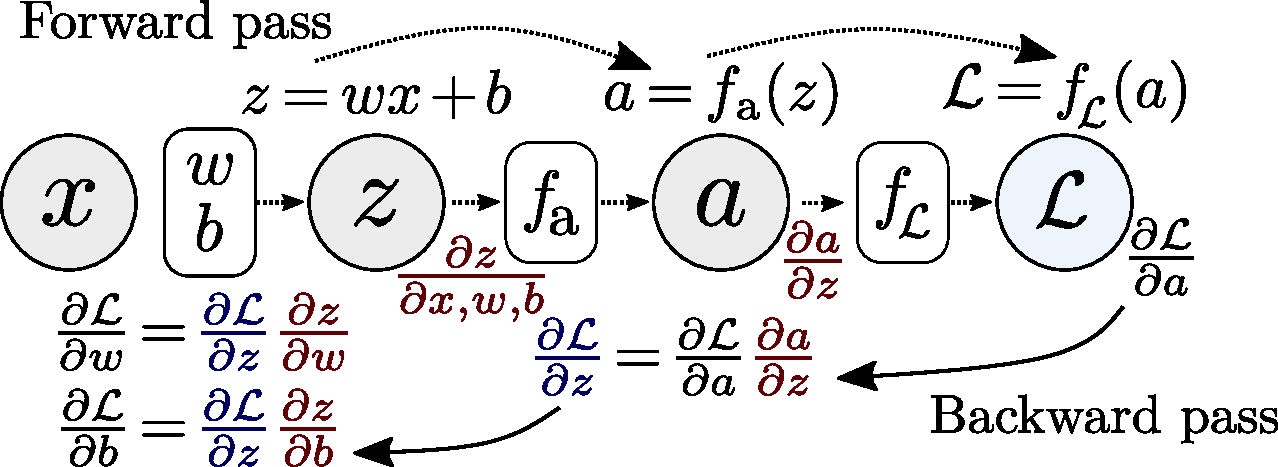
\includegraphics[width=0.80\linewidth]{vector/backprop-toy.pdf}
    \vspace{-3mm}
    \caption{The principles of backpropagation in a single-neuron toy network.}
    \label{fig:backprop-toy}
\end{figure}

For realistic cases we need the chain rule's vector generalization. Suppose $ \mathcal{L} \in \mathbb{R} $ is a function of $ \a \in \mathbb{R}^{n} $, which is in turn a function of $ \z \in \mathbb{R}^{m} $; we write this as
\begin{equation*}
    \mathcal{L} = \vec{f}_{\raisebox{-0.4ex}{\scalebox{0.7}{$\mspace{-3mu} \mathcal{L}$}}} (\vec{a}) = \vec{f}_{\raisebox{-0.4ex}{\scalebox{0.7}{$\mspace{-3mu} \mathcal{L}$}}} \big( \vec{f}_{\text{a}} (\z) \big),
\end{equation*}
where $ \vec{f}_{\raisebox{-0.4ex}{\scalebox{0.7}{$\mspace{-3mu} \mathcal{L}$}}} : \mathbb{R}^{n} \to \mathbb{R} $ and $ \vec{f}_{\text{a}} : \mathbb{R}^{m} \to \mathbb{R}^{n} $. Then the gradient of $ \mathcal{L} $ with respect to $ \z $ is
    \begin{equation*}
        \subgrad{\z} \mathcal{L} = \left( \pdv{\a}{\z} \right)^{\top} \mspace{-7mu} \cdot \subgrad{\a} \mathcal{L} \in \mathbb{R}^{m},
    \end{equation*}
    where $ \pdv{\vec{y}}{\vec{x}} \in \mathbb{R}^{n \times m} $ is the function $ \vec{f}_{\text{a}} $'s Jacobian matrix. In practice, one would use an even more general tensor formulation applicable to objects with an arbitrary number of indices. For scalar loss $ \mathcal{L} $ as a function of a tensor\footnote{Note that term tensor is used loosely here to mean an array-like object with elements specified by an arbitrary number of indices, which is not the precise mathematical definition of a tensor.} $ \tensor{A} $, in turn a function of a tensor $ \tensor{Z} $, this reads
\begin{equation*}
    \subgrad{\tensor{Z}} \mathcal{L} = \sum_{j} \big( \subgrad{\tensor{Z}} \tensor{A}_{j} \big) \pdv{\mathcal{L}}{\tensor{A}_{j}},
\end{equation*}
where $ j $ is a tuple index that runs over all possible indices into the tensor $ \tensor{A} $. Further discussion falls beyond our scope; interested readers are referred to Chapter 6.5 of Ref. \cite{goodfellow}.

\section{Additional Technical Details About CNNs} \label{s:appendix-cnn}

\subsection{Zero-Padding}
As was shown visually in Figures \ref{fig:conv-single-channel} and \ref{fig:conv-multi-channel}, the convolution process shrinks the input image along the spatial dimensions. In cases where this is undesirable, the input image is \textit{zero-padded}---zeros are appended to its border, artificially increasing the input's size, which in turn increases the size of the output. In practice, zero padding is often used to ensure a convolution's input and output have equal spatial dimensions.

% By appending an appropriate number of zeros, the convolution's output can be made to have any desired spatial dimensions. 

% \textbf{TODO:} {\color{red} add a diagram to visualize zero-padding and non-unit stride.}

\subsection{Stride}
Often, one might wish to convolve the kernel and image at, say, every other position in the image. In this case, the kernel slides across the input image multiple pixels at a time; the number of pixels between successive kernel positions is called \textit{stride}. Strides larger than one are equivalent to downsampling the input image, and are used to save on memory and computation cost for high-resolution images. For the interested reader, Ref. \cite{cnn-guide} provides intuitive visualizations and clear explanations of both zero-padding and stride.


\subsection{Convolutional Arithmetic} \label{ss:conv-arithmetic}
We now present the (straightforward) formalism describing how an inputted image propagates through the layers of a convolutional network. Like in \myhref{s:appendix-fcn}{Appendix \ref{s:appendix-fcn}} for FCNs, we begin by introducing the notation needed to describe a CNN.
\begin{itemize}

    \item Let $ C_{\text{in}} $ and $ C_{\text{out}} $ denote the number of channels in an input and output feature map, respectively.

    \item Let $ I_{\text{w}} $ and $ I_{\text{h}} $ denote the number of pixels in an input feature map along the width and height axes, respectively.

    \item Let $ K_{\text{w}} $ and $ K_{\text{h}} $ denote the number of pixels in a convolutional kernel. % along the width and height axes, respectively.

    \item Let $ O_{\text{w}} $ and $ O_{\text{h}} $ denote the number of pixels in an output feature map. % along the width and height axes, respectively. 

    \item Let $ p_{\text{w}} $ and $ p_{\text{h}} $ ($ p $ for ``padding'') denote the number of zeros added to the beginning and end of the input feature map's width and height axes, respectively.

    \item Let $ s_{\text{w}} $ and $ s_{\text{h}} $ denote the kernel's stride along the width and height axes.

\end{itemize}
As is straightforwardly seen in Figure \ref{fig:conv-single-channel}, the output shape $ O_{j} $ along the axis $ j \in \{\text{w}, \text{h}\} $, for input and kernel dimensions $ I_{j} $, $ K_{j} $ and for $ s_{j} = 1 $ and $ p_{j} = 0 $, is given by
\begin{equation*}
    O_{j} = (I_{j} - K_{j}) + 1.
\end{equation*}
More generally \cite{cnn-guide}, the output shape along the axis $ j $ for arbitrary $ I_{j} $, $ K_{j} $, $ p_{j} $ and $ s_{j} $ is
\begin{equation}
    O_{j} = \floor*{\frac{I_{j} + 2p_{j} - K_{j}}{s_{j}}} + 1, \label{eq:cnn-O-conv}
\end{equation}
where the vertical bars denote the floor function, used in case the stride $ s_{j} $ does not evenly divide the numerator. 

We can now fully describe the propagation of an input feature map through a convolutional layer. Suppose the layer's input feature map has the shape $ (C_{\text{in}}, I_{\text{w}}, I_{\text{h}}) $, and a set of $ C_{\text{out}} $ kernels with spatial dimensions $ (K_{\text{w}}, K_{\text{h}}) $ is used to process the input image. In this case, the convolutional layer's output has the shape $ (C_{\text{out}}, O_{\text{w}}, O_{\text{h}}) $, where the output dimensions $ O_{j} $ are found from Equation \ref{eq:cnn-O-conv}. This output can then be used as the input to a subsequent convolutional layer with a different set of kernels, and the convolution process repeats in the next layer, as outlined in \myhref{ss:cnn-architecture}{Section \ref{ss:cnn-architecture}} on CNN architecture.

\newpage

% BEGIN REFERENCES PAGE
% --------------------------------------------- %
% decrease margins so references fit on a single page
\newcommand{\refhmargin}{2.65cm}
\newgeometry{left=\refhmargin, right=\refhmargin, top=3.0cm, bottom=3.0cm}

\fancypagestyle{referencestyle}{  % include page number only
\fancyhf{}
\fancyfootoffset[R]{0cm} % this resets centered page number after \newgeometry, not sure of the underlying theory but it works
\fancyhead[L]{\textit{\firstleftmark}}
\fancyfoot[C]{\thepage}
}
\thispagestyle{referencestyle}
\printbibliography
% --------------------------------------------- %
% END REFERENCES PAGE

\end{document}
